\documentclass{IEEEtran}
\usepackage{fontspec}

\newfontfamily\aplfont[Scale=0.90]{APL385.ttf}
\setmonofont[Scale=0.90]{APL385.ttf}

\usepackage{graphicx}
\graphicspath{{assets/}}
\usepackage{glossaries}
\usepackage{listings}
\usepackage{threeparttable}
\usepackage{todonotes}
\usepackage{soul}

\usepackage[absolute]{textpos}

\usepackage[style=ieee]{biblatex}
\usepackage{listings}
\addbibresource{main.bib}

\newacronym{API}{API}{application programming}
\newacronym{DSP}{DSP}{digital signal processor}
\newacronym{SDN}{SDN}{software defined networking}
\newacronym{NFV}{NFV}{network function virtualization}
\newacronym{CRI}{CRI}{container runtime interface}
\newacronym{IR}{IR}{intermediate representation}
\newacronym{Wasm}{Wasm}{WebAssembly}
\newacronym{BIOS}{BIOS}{basic input/output system}
\newacronym{BPF}{BPF}{Berkeley Packet Filter}
\newacronym{GPU}{GPU}{graphics processing unit}
\newacronym{PTX}{PTX}{Parallel Thread Execution}
\newacronym{LLVM}{LLVM}{Low Level Virtual Machine}
\newacronym{GPGPU}{GPGPU}{general-purpose computing on graphics processing units}
\newacronym{GLSL}{GLSL}{OpenGL Shading Language}
\newacronym{CUDA}{CUDA}{Compute Unified Device Architecture}
\newacronym{DSL}{DSL}{domain-specific language}
\newacronym{SIMD}{SIMD}{single instruction, multiple data}
\newacronym{SPIR-V}{SPIR-V}{Standard Portable Intermediate Representation V}
\newacronym{COTS}{COTS}{commercial off-the-shelf}
\newacronym{SoC}{SoC}{system on a chip}
\newacronym{SSA}{SSA}{static single assignment}
\newacronym{MSL}{MSL}{Metal Shading Language}
\newacronym{MEC}{MEC}{Multi-access Edge Computing}
\newacronym{APL}{APL}{A Programming Language}
\newacronym{CPU}{CPU}{central processing unit}
\newacronym{AVX}{AVX}{Advanced Vector Extensions}
\newacronym{RF}{RF}{random forest}
\newacronym{NF}{NF}{network function}
\newacronym{DNS}{DNS}{domain name system}
\newacronym{CNI}{CNI}{container network interface}

\lstdefinestyle{mystyle}{
    basicstyle=\aplfont\footnotesize,
    breaklines=true,
    numbers=left,
    numbersep=3pt,
}
\lstset{style=mystyle}

\usepackage{titling}
\renewcommand\maketitlehooka{\null\mbox{}\vfill}
\renewcommand\maketitlehookd{\vfill\null}

\begin{document}

\begin{titlepage}
    $ $ % very important line do not remove
    \vspace{7cm}
    \begin{center}
        \huge{Leveraging APL and SPIR-V languages to write network functions to be deployed on Vulkan compatible GPUs}
    \end{center}    
    
    \begin{figure*}[ht]
        \centering
        \begin{minipage}[b]{0.25\textwidth}
            
\includegraphics[width=\textwidth]{ul.png}
        \end{minipage}
        \quad \quad %%
        \begin{minipage}[b]{0.25\textwidth}
            
\includegraphics[width=\textwidth]{inria.png}
        \end{minipage}
    \end{figure*}
    
    \begin{textblock}{200}(10,12)%
    \obeylines
    \setlength{\parskip}{0cm}
        University of Lorraine
        Master of Computer Science - MFLS
        Master's Thesis
        Juuso Haavisto
        Supervisor: \textit{Dr.} Thibault Cholez
        Research Team: RESIST
        \today
    \end{textblock}%
    
\end{titlepage}

\tableofcontents

\newpage

\begin{abstract}

Present-day computers apply parallelism for high throughput and low latency calculations. However, writing of performant and concise parallel code is usually tricky.

In this study, we tackle the problem by compromising on programming language generality in favor of conciseness. As a novelty, we do this by limiting the language's data structures to rank polymorphic arrays. We apply our approach to the domain of Network Function Virtualization (NFV). We use GPUs as the target hardware. This complements NFV research in replacing purpose-built hardware with commodity hardware. Further, we present an empirical case study of a random forest implementation used to classify network traffic. We write the application for GPUs with SPIR-V Intermediate Representation (IR) while using APL as a modeling language.

To our knowledge, this approach is novel in three ways. First, SPIR-V has not yet been demonstrated to be used in machine learning applications. Second, we translate a non-imperative language APL to SPIR-V GPU IR. Using a non-imperative source language for GPUs is rare in general. Third, we show how SPIR-V programs can be used in Kubernetes microservice orchestration system. This integrates our proposed parallel computation pipeline to industry NFV deployment standards. 

We benchmark the SPIR-V code against C with a random forest of size 150x6000x300. We find 8-core CPU runtime to average 380ms and RTX 2080 GPU to average 480ms. Hence, space is left for further improvements in future work, which we detail for both the GPU pipeline and APL to GPU compilation.

\end{abstract}

\newpage

\section{Introduction}

In the software industry, progress in computation capability has historically followed Moore's law. While it is an open debate whether Moore's law still holds, it's without a doubt that classical computer architectures have evolved to multi-core. To elaborate, commodity computers in the 20th century were single-core systems. This paradigm saw a big change at the start of the 21st century. During the first decade, the physical core count started to increase rapidly. First came the dual-core processors: in 2001, IBM \textit{POWER4} became the first commercially available multi-core microprocessor. Similarly, AMD released their first dual-core system in 2005 under brand name \textit{Athlon 64 X2}, and Intel released \textit{Core Duo} processor series in 2006. Core count has then kept on steadily increasing on each microprocessor release: in 2020, the flagship consumer multi-core processor from AMD, called \textit{Ryzen Threadripper 3990X}, has 64 physical cores and 128 logical threads. Moreover, in the \gls{GPU} landscape, the difference is even larger. E.g., in 2005 a Nvidia flagship GPU model \textit{GeForce 6800 GT} had 16 cores for pixel shaders. In 2020, a \textit{GeForce RTX 2080 Ti} sports 4352 shader processors. 

Yet, despite the hardware changing, most programmers still think of software from the viewpoint of a single thread. Performance-wise this is suboptimal, as it means that the way software benefits from multi-core systems are dependant on the smartness of the compiler. Further, as parallelism is abstracted from the programmer, it is easy to construct data-and control-structures which result in execution logic that cannot be safely parallelized, or parallelized without much performance gain compared to single-core processing.

As such, an open research question remains: how parallel software could be better programmed? Coincidentally, this is the topic of this study. In particular, we focus on \glspl{GPU}. \glspl{GPU} have recently found use as a general-purpose computation accelerator for programs with high parallelisms, such as machine learning. Here, the data structures of these programs tend to be based on arrays: languages which encode software for \glspl{GPU}, e.g., Futhark \cite{Henriksen:2017:FPF:3062341.3062354}, is based on the purely functional array programming paradigm. But, we take the array programming paradigm a step further, inspired by \gls{APL} \cite{hui2020apl}, which only permits array data structures. To achieve such semantic in practice, we translate our program into \gls{SPIR-V}. \gls{SPIR-V} is the current technological spearhead of \gls{GPU} \gls{SSA} \glspl{IR}. Our thesis is that by combining the language and the execution environment to only match the usual computation domain tackled with \glspl{GPU}, we could better reason about such programs. As such, this directly addresses the problem of efficient use of current computation hardware. Should it be possible to implicitly parallelize all computations while enforcing parallel program construction, we could ensure that software runs as fast as physically possible. To our knowledge, this is the first attempt at creating a compute \gls{DSL} on top of \gls{SPIR-V}.

The study is organized as follows: first in §\ref{ch:bg}, we present a literature review. The review considers cloud computing models, and programming language approaches to achieve parallelism. After this, we move onto the empirical part in §\ref{ch:contribution}. First, in §\ref{ch:p2a}, we select a machine learning application written in Python and look at how it uses a C-language sub interpreter to produce parallel code for \glspl{CPU}. The selected machine learning application considers \gls{NFV}, i.e., use-case in which machine learning models are used for network processing. The machine learning application in question comes from a previous paper \cite{brissaud2019transparent} of the research group under which this study was conducted. Next, we manually translate its Python-and-C implementation into \gls{APL}. The APL code we then manually translate into \gls{SPIR-V}. Some technical details of the SPIR-V translation are presented in §\ref{ch:prgspirv}. Next, in §\ref{ch:sysarch} we present the \gls{GPU} system architecture. In §\ref{ch:k8s}, we start with the high-level view of how a Vulkan-based \gls{GPU} bootloader. We describe how the loader can be integrated as a microservice in today's de-facto industrial cloud computing framework called Kubernetes. The loader program in itself, which leverages a systems programming language Rust and a low-level Vulkan \gls{API} to control the \gls{GPU}, is described in §\ref{ch:loader}. After this, in §\ref{ch:results} we benchmark the \gls{SPIR-V} against the Python-C implementation. This marks a performance comparison between a CPU and GPU processing for the machine learning application. Yet, we concede to the fact that the comparison is not evenly-leveled: the CPU is given a headstart due to a small sample size. We consider this an acceptable limitation in our research. This is because it contributes to a tangential research question about whether latency-sensitive computing, here, \gls{NFV}, can be accelerated with \glspl{GPU}. Following the results, in §\ref{ch:dicussion}, we contribute our findings on how our loader program and APL to SPIR-V compilation could be improved.  Finally, the study is concluded in §\ref{ch:conclusion}. 

\section{Previous research}
\label{ch:bg}

In the introduction, we pointed how computer programming has changed in the past 20 years in the form of parallelity: multi-processor CPUs have become ubiquitous, and GPUs are in increasing effect used for highly parallel workloads in domains of machine learning, where thousands of cores are used to solve tasks. Similarly, the way software is architected and turned into consumer services has also changed. Early worldwide web applications were widely architected as a client-server model with so-called monolithic application architecture. Here, monolithic applications mean that a single program did all possible computations required by the service and was likely run on a single dedicated server computer. While the client-server model has remained the standard during this century\footnote{Although, the term is now called "cloud"}, architectures have seen a proliferation towards microservices, which run in cloud computing environments. Such microservices are globally distributed within the cloud provider network, and provisioned inside resource isolated containers \cite{burns2016borg} and, as of more recently, inside virtual machines with formal semantics \cite{haas2017bringing, watt2018mechanising}. In general, computing can be seen to have higher execution granularity than before, shifting from a single computer execution towards distributed execution of highly parallelized individual threads. For example, in \cite{fouladi2017encoding}, video processing is split among thousands of tiny threads across many physical servers. Similarly, the Ethereum project is an attempt at a so-called world computer concept. In accordance with the microservice trend, Ethereum has software "contracts," which are executed among multiple computers to form a consensus of the world's computer state. However, both in Ethereum and in the cloud there exists open safety challenges: it is 1) hard for programmers to formally reason about the distributed execution of their code, and 2) it is hard to ensure that the scheduler does not leak confidential data when resources are re-used \cite{jangda2019formal} or that the scheduler is fair.

It could be considered that software that is architected to be distributed is called cloud-native. In the following subsections, we further inspect different ways to comprise microservices that yield to this concept.

\subsection{Microservice Runtimes}

Microservice, as a term, has a loose definition. For the sake of simplicity, in our study, we do not consider the social aspects, but instead how the definition changes depending on what the underlying technical runtime is. To elaborate on the problem statement: a microservice with a container runtime runs a whole operating system on each container. As such, container-based microservices have very lax technical limitations. This is because an operating system has many processes, and in the end, a microservice will be a process. But this introduces a problem. Since the operating system can essentially an arbitrary amount of processes, a single container may be compromised of multiple microservices. While an organization can decide that each process that is not a vital operating system process is a microservice, sometimes such an approach is impractical. For example, a program may have a proprietary dependency that may not listen to network ports. In this case, a process-based definition for a microservice would not work.

In general, it could be considered that when a microservice runtime is not restrictive, it becomes a social problem to define it. As the following subsections will show, some technical approaches have emerged which are more restrictive. Here, the program granularity is reduced from the container's process towards a lambda function. For the sake of conciseness, we evaluate what we consider widely known approaches of microservice runtimes, shown in Fig. \ref{tb:runtimes}.

\begin{table*}
\begin{center}
\caption{Microservice runtimes}
\begin{tabular}{ c|c|c|c } 
 Technology & Overhead & Application Capabilities & Orchestrator \\
 \hline
 VM & Full OS + Full OS & Full OS & e.g., Xen \\ 
 Containers & Full OS + Partial OS & Full OS & Kubernetes \cite{burns2016borg} \\ 
 Unikernels & Partial OS  & Full OS & e.g., iPXE  \\ 
 Serverless & Full OS + WASM Runtime  & A function & e.g., Lucet \\
\end{tabular}
\end{center}
\label{tb:runtimes}
\end{table*}

\begin{table*}
\begin{center}
\caption{NFV acceleration methods}
\begin{tabular}{ c|c|c|c|c } 
 Technology & DSL & Overhead & Application Capabilities & Orchestrator \\
 \hline
 GPUs & e.g., SPIR-V & Full OS + Graphics API + GPU & A chain of functions & e.g., Legate \cite{bauer2019legate} \\
 Linux kernel passthrough & e.g., BPF & Any deployment method on Linux & A chain of functions &  \\
 FPGAs & e.g., P4 & Specialized hardware & A chain of functions & \\
\end{tabular}
\end{center}
\end{table*}

\subsubsection{Containers}

Arguably the most well-known packaging format of software is currently containers, which developers usually interface via Docker or some other \gls{CRI}. As containers focus on isolation and dependency minimization of arbitrary software, it makes them a compelling basis for microservices. In the abstract, the idea is that the developer creates a reproducible and self-contained build-script for their applications from a clean-slate operating system installation. This way, the developer may install any software required to run their application while also making a reproducible build system that allows restarts and migrations of the container. Such features are relevant, as containers nowadays often run with orchestration systems such as Kubernetes \cite{burns2016borg}. Such orchestration systems claim to make managing containers to equal managing applications rather than machines \cite{burns2016borg}, simplifying development operations, and pooling all computation capabilities into a single uniform abstraction. Further, these abstractions enable the software development process to be streamlined and simplified from the viewpoint of the developer: in our previous studies, e.g., \cite{haavisto2019open}, a Kubernetes-based installation is coupled with a version-control integrated deployment process. Such abstraction then even abstracts away the whole concept of computing resources, which might, in turn, help developers focus on business goals better. Especially in the industry, a promise of a universal solution to deploy software to production becomes compelling: according to \cite{burns2016borg}, containers isolate applications from operating systems, making them possible to provide the same deployment environment in both development and production, which, in turn, improves deployment reliability and speeds up development by reducing inconsistencies and friction.

Generally, containers are lightweight and fast: a single server can have hundreds of containers running \cite{amaral2015performance}. Yet, containers also produce overhead in the form of nested operation systems. Such challenges are to be considered, especially for performance-centric microservices architectures and, in our case, intensive I/O processing from network interfaces. To elaborate, should one rent a virtual server from a cloud provider such as Amazon, they already operate above an abstraction as cloud providers tend to rent only virtualized environments for customers. On top of this abstraction, a container-based approach requires an installation of the so-called host operating system (e.g., Ubuntu), on which the actual containers (e.g., Alpine Linux) are run. As such, a containerized application can quickly end up operating on top of three separate operating systems, each having their overhead. This may be challenging, especially for networking: one study concludes that containers decrease network performance by about 10\% to 20\% compared to bare-metal (i.e., non-nested container) deployments \cite{kratzke2017microservices}.

\subsubsection{Serverless}

When it comes to modern microservice runtimes, the serverless paradigm is the most recent and finer in granularity: here, the packaging format is a single function instead of the whole operating system. Such an approach has some interesting traits: it has significantly less overhead than containers, which make serverless applications much faster to respond to actions even if scheduled just-in-time. For example, the Amazon Firecracker scheduler has boot times of around 150ms \cite{agache2020firecracker} compared to seconds that it might take for a container on Kubernetes to start. The so-called fast cold-start time is relevant when thinking about more distributed and performance-orientated microservice architecture: the orchestrator may free memory and cycle capacity by turning off serverless applications which are not receiving traffic. And as soon as one receives a request, it can be started by almost imperceptible boot-up time. From a pragmatic perspective, it is also cost-efficient: a serverless application may sleep and start on-demand and also billed that way.

Yet, some studies, such as \cite{hellerstein2018serverless}, argue that the serverless paradigm is "one step forward, two steps back." One argument concerns the packaging method, i.e., the \gls{IR}, of serverless applications: with containers, the Dockerfile became the de-facto manifest format to declare container installations, which in itself resemble bash scripts by almost one-to-one. Yet, with serverless applications, it may be a bigger social problem to agree on how functions should be written. This problem directly stems from the fact that with containers, any language that can be installed on any operating system works, but with serverless, the users will likely become restricted on a single language. While there already exists papers of envisions of what the serverless paradigm will become, e.g., \cite{jonas2019cloud}, we denote that language-independent \glspl{IR} are gaining a foothold in the industry in the form of \gls{Wasm} \cite{haas2017bringing}. In abstract, \gls{Wasm} remarks a general shift from build-script approaches of packaging software towards a compiler-driven approach, in which the compiler backend produces \gls{Wasm} code instead of architecture-dependent bytecode. Originally, \gls{Wasm} was engineered to create faster and more heterogeneous JavaScript, but the paralleling usefulness as a non-hardware specific \gls{IR} and the requirement of such in the serverless paradigm is an apparent and promising fit.

\subsubsection{Unikernels}

A stark difference to the abstraction-heavy container and serverless approach is unikernels. Unikernels address both the performance pitfalls of layered kerneling of containers and can be used to avoid restricted language support of serverless by packaging software as Linux kernels \cite{raza2019unikernels}. For example, MirageOS \cite{imada2018mirageos} supports only application written in OCaml, whereas Rumprun [cite] is a reduced version of NetBSD, and as such, supports NetBSD compatible programming languages. In general, the unikernel approach means taking a constrained application environment, and packaging it as a Linux kernel \cite{raza2019unikernels} while stripping away operating system capabilities unnecessary to the program. Relevant to our use of microservices, this also means that performance-wise, kernel-passthrough approaches such as \gls{BPF} are not required for solely performance reasons, as the application already runs in kernel-mode. Further, unikernels make applications generally faster by running in privileged mode, as a lot of performance-degrading bagging, which comes from Linux security architecture to support a safe multi-user paradigm, is set aside. Considering the orchestration of unikernels, i.e., the deployment on a scale, to our understanding, no de-facto method exists, yet we see no reason why networked \gls{BIOS} bootloaders like netboot [cite] would not work.

\subsubsection{Executing microservices on GPU}

Network-processing has also been researched to be accelerated using \glspl{GPU}, e.g., via PacketShader \cite{han2010packetshader}. Here, the idea follows that computation tasks that concede well under the physical constraints of \glspl{GPU} are offloaded to a \gls{GPU}. This so-called \gls{GPGPU} paradigm has recently found its foothold in the form of machine learning applications, where especially neural networks concede well to the physical constraints of \glspl{GPU}, which include a limited and relatively slow uniform memory and MapReduce-like state synchronization. Hence, it can be concluded that in the grand scheme of general computation paradigms, \glspl{GPU} follow the general direction of distributed state like container deployments (MapReduce-like state synchronization) and also the thread-granular parallelism principles of serverless applications (slow uniform memory enforces parallelism), but here within a single physical component. As such, \glspl{GPU} can also be thought of as a microservice runtime, especially given support from an orchestrator such as Legate \cite{bauer2019legate}.

Yet, historically the \gls{GPGPU} standards and approaches have been dispersed at best: it remains commonplace to still use shading languages like \gls{GLSL}, meant to display graphics on a monitor, to be tricked into computing matrix algebra by using a no-display-producing graphics pipelines. There also exists an open standard \gls{API} called OpenCL, meant solely for computation workloads, but the standardization is not only meant for GPUs, but also for CPUs and FPGAs. Further, some \gls{GPU} manufacturers, such as Nvidia, have a proprietary \gls{IR} like the \gls{PTX} which is produced by Nvidia's \gls{CUDA} \gls{API} and as a backend target by the \gls{LLVM} compiler infrastructure to offer generally the most performant \gls{GPGPU} code available today. However, \gls{PTX} only works on Nvidia \glspl{GPU}. Coincidentally, this also means that programming models for \glspl{GPU} are also scattered: historically, the only options have been either open standards like OpenCL C or \gls{GLSL}, or then manufacturer-specific languages like \gls{CUDA}. Somewhat surprisingly, the programming model of these most common \gls{GPGPU} languages is imperative, whereas it has been commonplace for CPUs to have \glspl{DSL} with formal foundations on concurrency primitives like communicating sequential processes \cite{hoare1978communicating} on recent languages for multi-core environments like Erlang or Go.

More recently, the open \gls{GPU} standards working group called Khronos, which is the organization behind \gls{GLSL} and OpenCL, among many other open initiatives in the \gls{GPU} space, has released \gls{GPGPU} enablers to a new cross-platform graphics \gls{API} focused on performance, called the Vulkan \gls{API}. These new capabilities include a cross-platform formally verified memory model called the Vulkan memory model (further introduced in §\ref{ch:vmm}), and a class of cross-platform \gls{SIMD} operands for non-uniform group operations called subgroups (further introduced in §\ref{ch:vso}). Yet, the Vulkan \gls{API}, while released in 2016, has not seemingly become the leading \gls{API} so far in the \gls{GPGPU} space, plausibly affected by a design decision to only support a new open standard \gls{IR} called SPIR-V. As such, any application which wishes to adopt Vulkan's features would first need to update all the \gls{GPU} code to \gls{SPIR-V}, which in practice is done via cross-compilers which may not necessarily translate the most performant code. Further, some of the features, such as the Vulkan memory model was released as recently as September 2019. We deem it likely that most translators will require more time to adopt. As such, as a consistent memory model is paramount for deterministic computation results, it can be considered no subject of wonder why the technology adoption may have been slow. Finally, regarding microservices, a previous paper of ours \cite{haavisto2020interoperable} studied the Vulkan and SPIR-V powered \gls{GPGPU} paradigm in light of cold-start times and interoperability: it was found that the 99th percentile for starting the same programs was $1.4$ms for a \gls{COTS} desktop GPU (Nvidia RTX 2080), and $4.3$ms for ARM-based \gls{COTS} mobile \gls{SoC} (Nvidia Jetson TX2). So, in terms of cold-start times, this places a modern \gls{GPGPU} microservice latency to the similar ballpark as serverless applications hence significantly faster than containers.

\subsection{Hardware acceleration for parallel computing}

\begin{figure*}
  \centering
  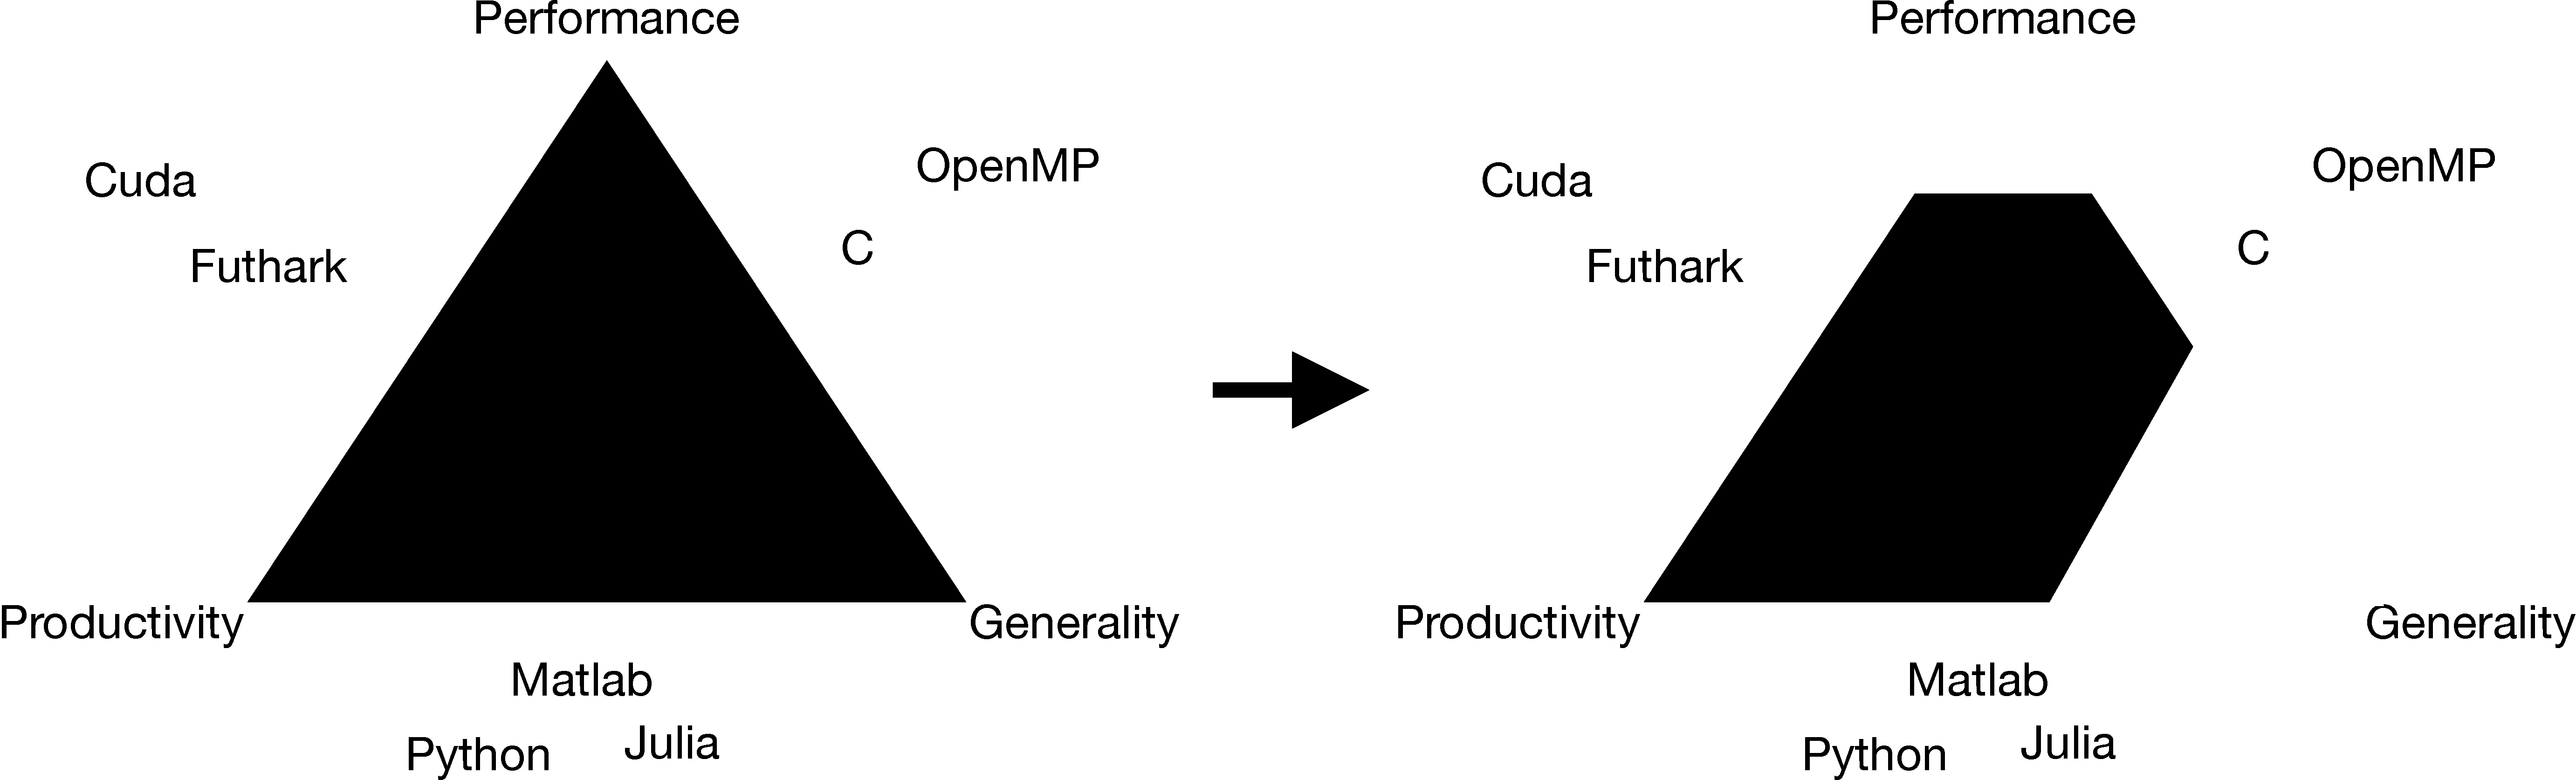
\includegraphics[width=\columnwidth*2]{tric}
  \caption{How programming languages and approaches for machine learning are made faster: by removing generality and by compromising on utmost performance. (Model inspired by \cite{brown2011heterogeneous})}
  \label{fig:tri0}
\end{figure*}

When thinking about programming languages to develop microservices, we can think of an abstraction shaped like a triangle, shown in Fig. \ref{fig:tri0}. On the left, we can see how programming languages are located in different parts of the triangle, portraying their focus on solving problems. For example, C is considered general and highly performant. However, C is not considered very productive because it allows a class of bugs to happen, which are not possible in other languages. On the other hand, scripting languages like Python, which are oftentimes used in machine learning, are not very fast, but as a plus have general problem domains and are arguably easy to program. On the left side, we have languages that are not very general, i.e., they require separate computing accelerator devices like GPUs to work, but yet for that reason are easier to program for domain-specificity. Hence, such languages can assume more about the programming style than in CPU-languages. Further, GPU languages do not have filesystem, network, or persistent storage access. As such, reasoning about accelerator languages can be considered easier, as unpredictable sources of infinite input and output, e.g., file descriptors, do not exist.

Yet, it is also noteworthy to recognize that many approaches exist in accelerating the languages found from the bottom side of the triangle can be "lifted." By lifting, we mean there exist approaches for these languages which move them towards the center of the triangle. In our concept, a language that is at the center of the triangle is considered an ideal programming language. But how does this lifting work? In this section, we focus on some of such approaches, namely 1) advanced vector extensions, 2) general-purpose computing on graphics processing units.

\subsubsection{Advanced Vector Extensions}

\gls{AVX} can be considered the general method of accelerating programming languages on today's hardware. AVX achieves this by only operating on a subset of programs, which yield to \gls{SIMD} instructions— in a sense, considering Fig. \ref{fig:tri0}, \glspl{AVX} can be efficiently applied when generality is cut down to only consist of array operations and data-parallel data structures. Coincidentally, as a result of domain-specificity of AVX on \gls{SIMD}, the triangle gets sliced from the angle of generality. In practice, this angle-slicing effect is usually applied to languages through scientific computing libraries, which essentially only include matrix algebra in them. For example, in Python, the NumPy library is such a domain-restricted library.

Once a library like NumPy is used, what essentially happens is that a sub interpreter or just-in-time compiler gathers the program calls, which are compiled down to platform-specific bytecode. This produced bytecode is then the format on which the SIMD instructions have been applied. Yet, as the bytecode generation is platform-specific, libraries like OpenMP exist. These abstractions aim to compile the code to run as fast as possible regardless of the platform. In practice, most of these libraries leverage the \gls{LLVM} compiler project to detect and interoperate on a single shared \gls{IR}. As seen, e.g., in Numba \cite{lam2015numba}, the LLVM IR is useful because as in some cases, it allows a single IR to be compiled to vector instruction accelerated \gls{CPU} and \gls{GPU} code.

\begin{figure}
  \centering
  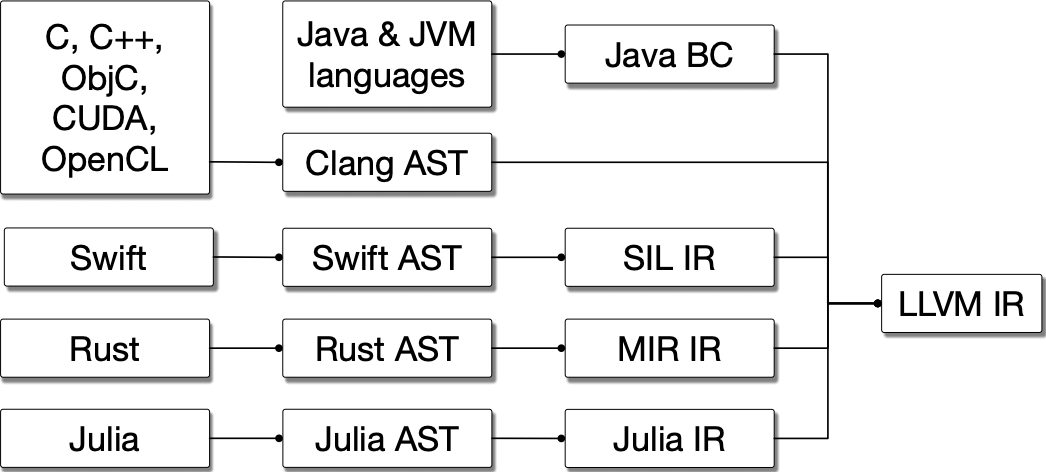
\includegraphics[width=\columnwidth]{mlir.png}
  \caption{Compilation pipeline of different languages with multiple mid-level IRs for language specific optimization with common backend for multiple hardware targets. Source: \cite{lattner2020mlir}}
  \label{fig:mlir}
\end{figure}

As of very recent, the power of shared IR and the shared compiler has also been applied to domain-specific purposes itself, here, to deep neural networks, as in MLIR \cite{lattner2020mlir}. As such, MLIR can be considered a problem-domain specific \gls{SSA}-based IR for heterogenous target platforms, which include CPU, GPU, tensor programming unit (TPU), and "others." We believe that this notion of compilers having more features and compiler passes is interesting, as pictured in Fig. \ref{fig:mlir}. That is, in recent languages like Swift, Rust, and Julia, further compiler passes allow the developers to write compiler extension libraries in the original language. In specific, this mid-level pass is one that has passed the type-checker but has not yet generated SSA code. As such, it seems generally prosperous future development that the proliferation of more compiler passes will help to move traditionally slow languages into faster ones without any further input from the software developer.

In practice, we generalize those speed improvements are achieved by effectively detecting code, which yields well to SIMD and data-parallelism. Further, array-orientated libraries like NumPy essentially function by exposing domain-specific pragmas to compilers, which are often tacit to the software developer.

\subsubsection{General-purpose computing on graphics processing units}
\label{ch:gpgpu}

\gls{GPGPU} is a similar approach as AVX in the sense that GPGPU revolves around a similar register-based programming style. However, this approach can be considered to be taken even further: in the GPGPU paradigm, the software is essentially written from the viewpoint of a single register. For example, in GPGPU, a vector sum is something like the following:

\begin{lstlisting}
lhs := float numbers[1, 2, 3, 4];
rhs := float numbers[4, 3, 2, 1];

main() {
    uint index = InvocationID.x;
    lhs.numbers[index] += rhs.numbers[index];
}
\end{lstlisting}

Here, we can see that the main function receives some undefined structure called \verb|InvocationID|, from which it takes a value of \verb|x|, which it uses as the index to add numbers between the vectors of \verb|lhs| and \verb|rhs|. As the main is ran only once, it would not be absurd to imagine the result of \verb|lhs| to be $[5, 2, 3, 4]$. Yet, in the GPGPU paradigm, the result is $[5, 5, 5, 5]$. This is because the main function is run per each \textit{invocation}, which resembles a thread. On a typical GPU, the maximum number of these invocations per program is usually very high. On yours truly laptop, the count is $1'073'741'823$.

Some programs which would traditionally require explicit loops, such as the vector sum defined above, are concisely presented in the GPGPU paradigm. However, some programs are much trickier. For example, the elementary operation of a sum reduction is hard because of the register-centric style. Here, a reduction either requires locking all other invocations while one of them scans through the rest. Alternatively, every invocation which's ID is odd would read its neighbors' value, and add it to self. Such a map reduction format happens to resemble much of the inner workings of neural nets, which has resulted in GPGPU being prolific in the machine learning space. In fact, much of the practical feasibility of neural network training nowadays comes from the fact that the GPGPU paradigm is available as an extension to languages like Python through languages like CUDA. A recent example of such work can be found from Nvidia Legate \cite{bauer2019legate}. In the paper, the authors show how Nvidia \gls{CUDA} is integrated with Python's scientific array programming library called NumPy in a convenient way, as shown in Fig. \ref{fig:legint}. Previous work to Legate also exist in form of CuPy \cite{okuta2017cupy} and Numba \cite{lam2015numba}. CuPy and Numba compare closely to Legate, but without inter-device work scheduling.

\begin{figure}
  \centering
  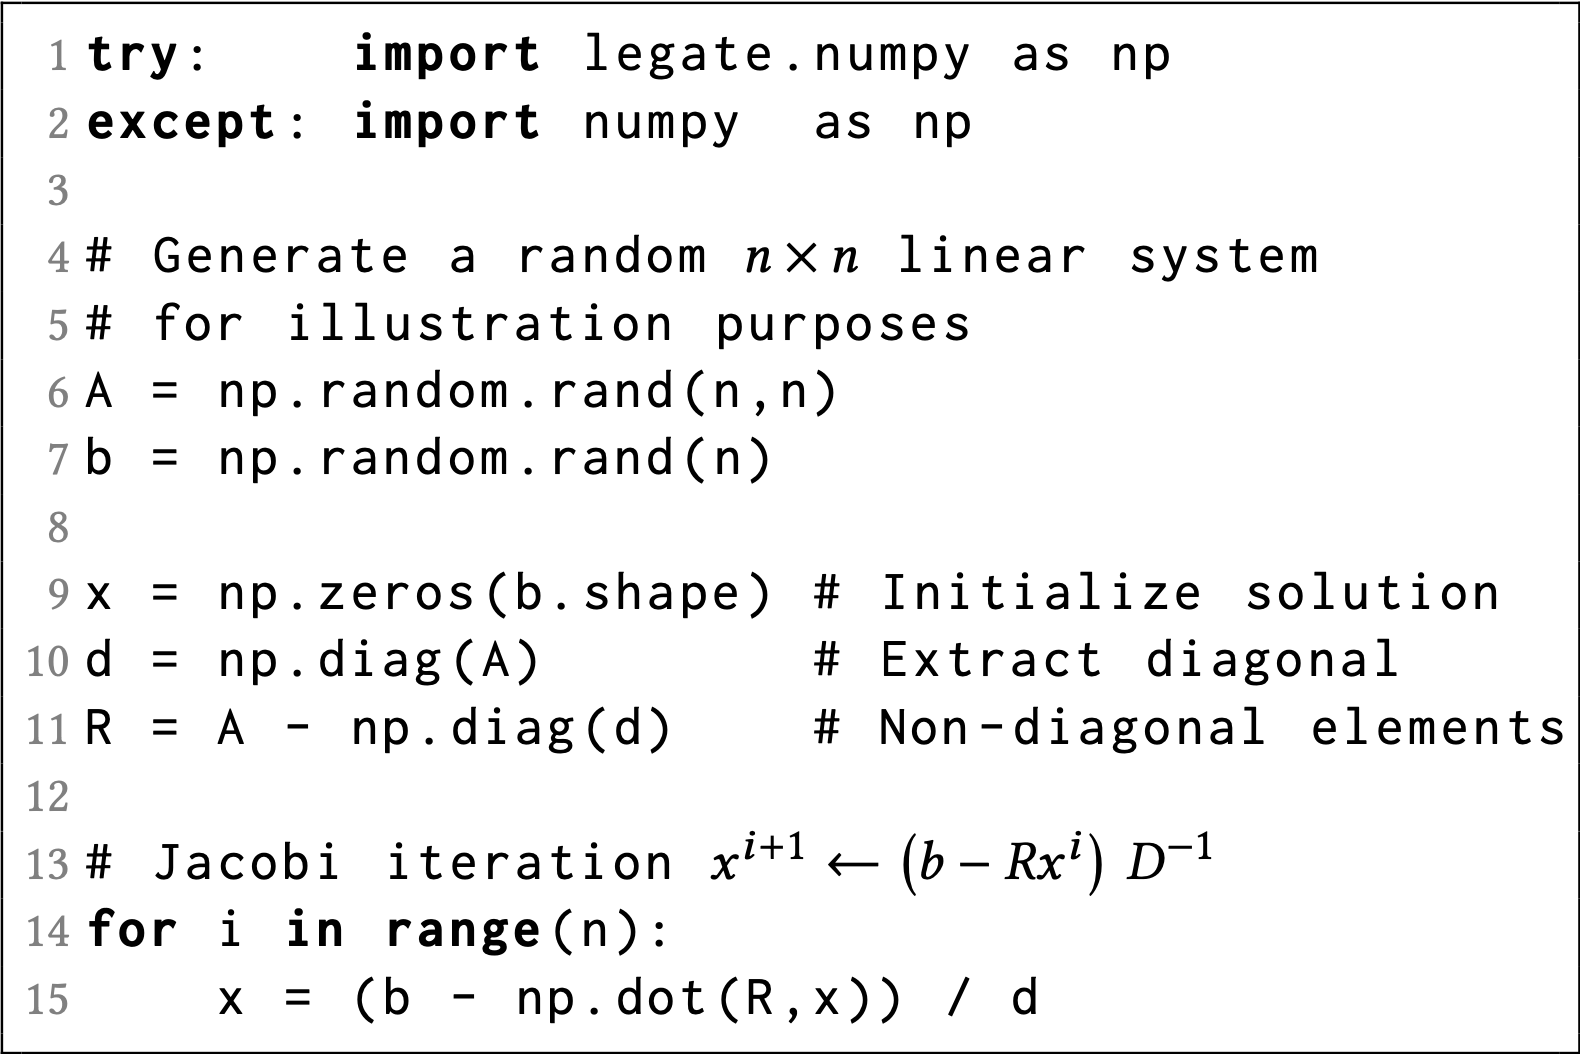
\includegraphics[width=\columnwidth]{legint.png}
  \caption{Sample code showing GPGPU paradigm seamlessly integrated into Python's NumPy. (Source: \cite{bauer2019legate})}
  \label{fig:legint}
\end{figure}

Projects like Legate, CuPy, and Numba are a prime example of performance "lifting" of productivity-focused languages like Python towards more complete triangles, per the mental model of Fig. \ref{fig:tri0}. Arguably, from the viewpoint of a developer who is satisfied with Python, the triangle is complete -- they have a) the performance of CUDA (if GPU is present) and b) if not, they are simply using CPU NumPy (which itself is accelerated with OpenMP on CPU), and c) they are using a language they feel is general and productive for them.

Given the possibility for the completeness of abstractions like Legate, it is no wonder that alternative approaches exist. For example, there exist GPGPU "lifters" for Matlab-like language Julia \cite{bezanson2017julia}. Some programmers may find languages like Julia better suited for their use-case, as the whole language is built on scientific computing. In specific, in Julia arrays and matrices as first-class, whereas in Python, such traits are imported via libraries like NumPy.

A differentiating take is Futhark \cite{Henriksen:2017:FPF:3062341.3062354} which is a functional programming language with GPGPU as language built-in feature. Interestingly, Futhark is able to represent the GPGPUs register-orientated computing paradigm in the functional programming paradigm, which is presented in the more traditional non-parallel computing approach. For example, average of a vector in Futhark is computed with:

\begin{lstlisting}
let average (xs: []f64) = reduce (+) 0.0 xs / r64 (length xs)
\end{lstlisting}

Here, it is worth noticing that the indices which would traditionally be required in the GPGPU paradigm are abstracted. Furthermore, some may find a functional programming style preferable over imperative approaches of Python and Julia.

\begin{figure}
\verb|      1 + 1|\\
\verb|2|\\
\\
\verb|      1 + 1 2 3 4|\\
\verb|2 3 4 5|\\
\\
\verb|      mat ← 3 3 ⍴⍳9|\\
\verb|1 2 3|\\
\verb|4 5 6|\\
\verb|7 8 9|
\\
\verb|      1 + mat|\\
\verb|2 3  4|\\
\verb|5 6  7|\\
\verb|8 9 10|

  \caption{APL examples here show rank polymorphism on plus operation over scalar, vector, and matrix. Note that looping is implicit. Also, note that APL is read right-to-left: definition of the mat is a reshape of $1..9$ vector over the left-hand-side argument, hence producing 3x3 matrix with values taken from range $1..9$.}
  \label{fig:apl}
\end{figure}

Another approach to achieve performance for parallel computing is to make the language the array programming library. A family of languages that do this is known informally as APLs, which are based on a 1962 paper \cite{iverson1962programming} by Kenneth Iverson (a recent historical view on the language is provided in \cite{hui2020apl}). In the paper, a language called A Programming Language for teaching matrix algebra was introduced. An interesting and distinctive aspect of APLs is that there is no explicit iteration or recursion in the standard\footnote{But, as we will later see, newer versions of APL do include explicit recursion.} \cite{isoapl}, but instead, operation ranks are automatically lifted to higher dimensions. This means that, e.g., plus operation works irrespective of the array rank, as demonstrated in Fig. \ref{fig:apl}. It has been argued \cite{slepak2014array} that such abstraction solves the so-called von Neumann bottleneck \cite{backus1978can} which complements Iverson's own argument for APL being "a tool of thought" \cite{iverson2007notation}. In abstract, APL proponents call the capability of rudimentary index operation abstraction as a programming approach that contributes to the correctness and brevity of computation solving. In other words, as less effort is put into thinking about programming paradigms, APLs free attention towards the original mathematical problem on-hand. More recently (e.g., see: \cite{hsu2019phd, slepak2014array}), APL's model of loop and recursion-free array processing has gained research interest as a way to simplify parallel computation. In specific, in \cite{hsu2019phd}, a data-parallel compiler was introduced. Here, it was shown that arrays could be used to represent abstract syntax trees. The produced compiler \cite{codfns}, called co-dfns, is able to produce C, \gls{CUDA}, and OpenCL code from a subset of APL when using the proprietary Dyalog APL interpreter. As such, the project ascends APLs usability to modern-day \gls{GPGPU} computing. We deem this as an interesting and fundamental development in terms of performance implications for \gls{GPGPU} code: as APL and its operands amount to simple matrix operations, then by forcing such array-based problem solving, it would force the developer to write automatically parallel code. As argued in length in \cite{mckenney2017parallel}, part of the reason parallel code is hard to write is that developers fail to understand the underlying hardware. As such, developers may unknowingly produce sequential algorithms and data structures and cause the hardware to compute redundancies, which slow computation. Redundancies include, e.g., using branch predictor over binary selector. According to Nvidia presentation \cite{harris2007optimizing}, elimination of branch prediction can increase throughput by 2x on GPUs.

% taichi_lang.pdf
% http://taichi.graphics/wp-content/uploads/2019/09/taichi_lang.pdf

% Many programming models for efficiently compiling array operations have been proposed.Halide [Ragan-Kelley et al.2012, 2013] decouples image process-ing operations and lower-level scheduling such as loop transforma-tions and vectorization. Several polyhedral compilers adopt a similaridea [Baghdadi et al.2015, 2019; Mullapudi et al.2015; Vasilacheet al.2018]. All these compilers focus on dense data structures anddo not model sparsity. Our language decouples algorithms from theinternal organization of sparse data structures, allowing program-mers to quickly switch between data organizations to achieve highperformance.Several sparse tensor compilers target linear algebra operations(e.g. taco [Chou et al.2018; Kjolstad et al.2017], ParSy [Cheshmi et al.2017, 2018]). They focus on constructing efficient iteration spacesbetween different sparse matrices under linear algebra operations.Several compilers target graph operations such as breath-first-searchor shortest path (e.g. [Wang et al.2016; Zhang et al.2018]). In con-trast, we focus on generating high-performance traversal code forspatially coherent access to hierarchical and sparse data structures.To efficiently vectorize access to data structures, we adopt theSingle-Program-Multiple-Data model [Darema et al.1988] in ourcomputational kernels, which is the foundation of modern parallel

% languages such as CUDA, OpenCL [Stone et al.2010], ispc [Pharrand Mark 2012], and IVL [Leißa et al. 2012].

% Inspired by the increasing relative expense of memory operations,the video game and visual effects industries have recently startedto adopt the data-oriented design philosophy [Acton 2014; Lee et al.2017]. It is a software engineering approach focused on data access,as opposed to the more traditional object-oriented design where thestorage is fragmented. Adopting a similar philosophy, ispc [Pharrand Mark 2012] and IVL [Leißa et al.2012] both provide constructsfor transformations between array of structures and structure ofarrays. Our language facilitates data-oriented design and sharesthe same philosophy through decoupling of data structures andcomputation.

\section{Contribution}
\label{ch:contribution}

\begin{figure*}
  \centering
  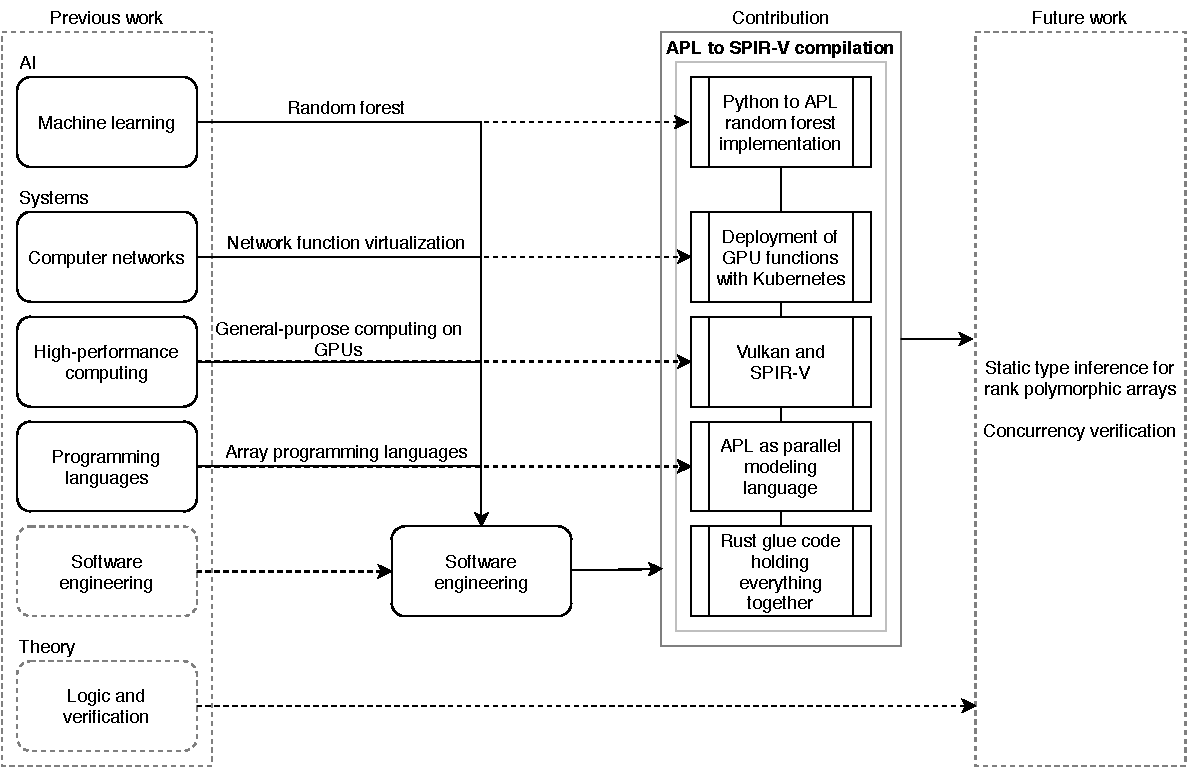
\includegraphics[width=\columnwidth*2]{overview.pdf}
  \caption{High-level overview of the research done in this study, and how they relate to previous work}
  \label{fig:ov}
\end{figure*}

With a brief introduction to programming languages and methods of hardware acceleration for parallel computation covered, we now focus on this study's focus. First, we present a high-level overview in Fig. \ref{fig:ov}. This figure details how we combine four different aspects (machine learning, computer networks, high-performance computing, and programming languages) in two different research branches (AI and systems) by using software engineering (which itself is a systems science) to produce a contribution which combines these aspects into one integrated process. Finally, we show that future work can be done to extend our hereby presented contribution with theoretical computer science by using logic and verification.

The context of our study is GPU microservices as a method to accelerate \gls{NFV}. We conclude from the previous research that GPU microservices are a timely subject because: 1) the new Vulkan API and SPIR-V IR can fix interoperability problems of past GPGPU approaches for microservices and 2) general trend in computation is towards parallelism and fine-grained programs, for which GPUs are a good fit for. Further, we decide to tackle the domain with APL. This is because we notice that fast parallelism is enabled by \gls{SIMD}, and APL introduces us to rank polymorphism. With rank polymorphism, APL can transform any operation to vectors, which may benefit from \gls{SIMD}. Additionally, APL forces us to think from an array-only mindset, which may produce unconventional but highly parallel approaches to solving existing problems. This, in turn, compliments our guest for new ways to do effective \gls{NFV} services by replacing purpose-built digital signal processors with commodity hardware such as GPUs. With the convoluted problem statement, we next move onto the empirical part of the study.

The empirical part of the work is a development to \cite{brissaud2019transparent}, in which \gls{RF} prediction is used to label encrypted hypertext data. We use the paper's application in this study by extracting the prediction algorithm as a GPU microservice, using the CPU implementation execution time as the baseline to improve on. We choose this application also because the binary decision tree traversed by \gls{RF} algorithms can be parallelized as each three is data-independent. Further, the amount of the trees to traverse is usually well above the amount of normal amount of logical threads that a CPU may have. As a thesis, such workload should see performance increase on GPUs, as the GPUs have thousands of cores. To elaborate, the physical processor of GPU is less likely to get throttled by its physical capabilities compared to its CPU counterpart, assuming that the execution time of the program takes long enough time. Henceforth, when referring to the "RF algorithm," or "our algorithm," we refer to this Python-based algorithm, which we will translate to SPIR-V in this study.

As mentioned, our approach to writing the GPU implementation is unusual: we rewrite the Python implementation in APL and use APL as a modeling language to write SPIR-V assembly code from. We argue that hand-writing APL operands in SPIR-V assembly are a worthwhile endeavor: APL is recently shown to produce well-parallelizable code \cite{hsu2016key} and its domain-specificity in array programming is already the base of modern machine learning libraries, such as NumPy, which we believe vouches for APL's fitness for machine learning acceleration. More importantly, APL as a language is comprised of only around 60 operations (albeit across four separate dimensions of scalar, vector, matrix, and cuboid), for which we deem it practically viable to offer hand-written SPIR-V implementation for each procedure. Further, we find some evidence that APL is strict enough to repel programmer constructions that diverge from parallel computation principles: the side-effects of zealous array programming, in specific, avoidance of explicit recursion and if-clauses (i.e., thread divergence), forces the programmer to write performant GPU code by default.

Yet, as GPUs are not typical computers, implementing all the operations for a full compiler is not without its eccentricities. As such, in §\ref{ch:prgspirv}, we describe some of the underlying peculiarities that affect GPUs.

Next, in §\ref{ch:k8s}, we notice that SPIR-V is a useful IR for another reason: the produced binary files are few kilobytes and can hence be inlined within text files. We use this finding to propose a way to orchestrate GPU \glspl{NF} on Kubernetes using Vulkan in the following subsections. 

\subsection{Python to APL translation}
\label{ch:p2a}

In this study, we use paper \textit{Passive Monitoring of HTTPS Service Use} \cite{brissaud2019transparent} as a case-study. The idea was to reimplement the \gls{RF} algorithm used for \gls{NFV} use-case on \gls{GPU}. We decided to use APL as a modeling language. In the end, we reimplemented three functions in APL:

\begin{enumerate}
    \item {\aplfont\begin{verbatim}
apply←{{
    i←⍵
    node←{⍵{(⍵+1)⌷,right[⍺;],left[⍺;]}⋄
    i(⍵⌷feature)⌷x≤⍵⌷th}while{⍵⌷left≠0}1
    out[i;]←node 1⌷values
}⍵}
\end{verbatim}}
    \item {\aplfont\begin{verbatim}
{{1⌷[2]↑⍒¨↓⍵(÷⍤1 0){⍵+0÷⍵}+/⍵}⍵}
\end{verbatim}}
    \item {\aplfont\begin{verbatim}
{a⊢←labels[⍵]@(∊∘⍵)a}¨∪res
\end{verbatim}}
\end{enumerate}

Here, the third item labels the result received from the second item. The second item normalizes and sums prediction values received by traversing the RF trees. The first item is the traversal algorithm of an RF tree, and coincidentally, it is the most computationally heavy function. In this study, we only implemented the full GPU reimplementation of the first item. This was because this function was the only part of the Python code which had C-optimizations. As such, it would be the only part which was accelerated in the Python version hence made a good comparison against a GPU implementation. Next, we describe our process of reimplementing the Python to APL and then to SPIR-V IR.

\textbf{Methodology} The debugger with pyCharm IDE was used to introspect the \verb|scikit| and \verb|numpy| models, from which \verb|numpy.savetxt| function was used to extract model files to a \verb|.csv| file. Using Sourcegraph, the \verb|scikit| \gls{RF} implementation\footnote{\url{https://sourcegraph.com/github.com/scikit-learn/scikit-learn@9358a6ee8f93511fd615d3264fa7ee9de0f21b93/-/blob/sklearn/ensemble/_forest.py#L673}}, \footnote{\url{https://sourcegraph.com/github.com/scikit-learn/scikit-learn@9358a6ee8f93511fd615d3264fa7ee9de0f21b93/-/blob/sklearn/tree/_classes.py#L916}} was refactored using the pyCharm debugger to produce APL program which produced the same result. We used Dyalog 17.1 IDE to test the APL code.

\textbf{Remarks} The APL program is model specific in the sense that it assumes the user only wants a single result. As such, there are no guarantees the same program works across all possible RF models which are compatible with Python. Yet, for the purpose of a simple case-study, we accept limiting the model output to 1 as fine.

\textbf{Translation} The first call to prediction is in the \verb|h2classifier| \verb|rf_tools.py| file. This file is part of our Github project\footnote{\url{https://github.com/toldjuuso/legendary-umbrella}}, which remains internal to Inria for the time being. Nevertheless, the file has a call as follows:

\begin{lstlisting}[language=Python]
pred_lab = clf.predict(feat_)
\end{lstlisting}

Where \verb|clf| is our model and \verb|feat_| are the samples. This call forwards to a function like this in:

\begin{lstlisting}[language=Python]
def predict(self, X):
    proba = self.predict_proba(X)
    
    if self.n_outputs_ == 1:
        return self.classes_.take(np.argmax(proba, axis=1), axis=0)
    
    else:
        n_samples = proba[0].shape[0]
        class_type = self.classes_[0].dtype
        predictions = np.empty((n_samples, self.n_outputs_),
                               dtype=class_type)
    
        for k in range(self.n_outputs_):
            predictions[:, k] = self.classes_[k].take(np.argmax(proba[k], axis=1), axis=0)
    
        return predictions
\end{lstlisting}

As our output size is 1, we only have to consider the first if-clause. But before that, the \verb|self.predict_proba(X)| calls the following:

\begin{lstlisting}[language=Python]
def predict_proba(self, X):
    check_is_fitted(self)
    # Check data
    X = self._validate_X_predict(X)
    
    # Assign chunk of trees to jobs
    n_jobs, _, _ = _partition_estimators(self.n_estimators, self.n_jobs)
    
    # avoid storing the output of every estimator by summing them here
    all_proba = [np.zeros((X.shape[0], j), dtype=np.float64)
                 for j in np.atleast_1d(self.n_classes_)]
    lock = threading.Lock()
    Parallel(n_jobs=n_jobs, verbose=self.verbose,
             **_joblib_parallel_args(require="sharedmem"))(
        delayed(_accumulate_prediction)(e.predict_proba, X, all_proba,
                                        lock)
        for e in self.estimators_)
    
    for proba in all_proba:
        proba /= len(self.estimators_)
    
    if len(all_proba) == 1:
        return all_proba[0]
    else:
        return all_proba
\end{lstlisting}

Here, we focus on the parallel code that Python evaluates, specifically this block:

\begin{lstlisting}[language=Python]
Parallel(n_jobs=n_jobs, verbose=self.verbose,
         **_joblib_parallel_args(require="sharedmem"))(
    delayed(_accumulate_prediction)(e.predict_proba, X, all_proba,
                                    lock)
    for e in self.estimators_)
\end{lstlisting}

The way this call should be interpreted is the following: for each \verb|e in self.estimators_|, calls the \verb|_accumulate_prediction| function, to which a function parameter \verb|e.predict_proba| among normal variables parameters \verb|X|, \verb|all_proba|, and \verb|lock| are passed. This brings us to the \verb|_accumulate_prediction| function, which looks like this:

\begin{lstlisting}[language=Python]
def _accumulate_prediction(predict, X, out, lock):
    prediction = predict(X, check_input=False)
    with lock:
        if len(out) == 1:
            out[0] += prediction
        else:
            for i in range(len(out)):
                out[i] += prediction[i]
\end{lstlisting}

Here, the \verb|predict| is now the function parameter of \verb|e.predict_proba|, which brings us to the next function:

\begin{lstlisting}[language=Python]
def predict_proba(self, X, check_input=True):
    check_is_fitted(self)
    X = self._validate_X_predict(X, check_input)
    proba = self.tree_.predict(X)
    
    if self.n_outputs_ == 1:
        proba = proba[:, :self.n_classes_]
        normalizer = proba.sum(axis=1)[:, np.newaxis]
        normalizer[normalizer == 0.0] = 1.0
        proba /= normalizer
    
        return proba
    
    else:
        all_proba = []
    
        for k in range(self.n_outputs_):
            proba_k = proba[:, k, :self.n_classes_[k]]
            normalizer = proba_k.sum(axis=1)[:, np.newaxis]
            normalizer[normalizer == 0.0] = 1.0
            proba_k /= normalizer
            all_proba.append(proba_k)
    
        return all_proba
\end{lstlisting}

Again, we have to only consider the if-clause in which the number of outputs is one, but before that, the function \verb|self.tree_.predict| is called. This brings us to the next function:

\begin{lstlisting}[language=Python]
def predict(self, *args, **kwargs): # real signature unknown
    """ Predict target for X. """
    pass
\end{lstlisting}

Here, we see that the call-stack "disappears" but in fact, this means we are calling Cython, which is Python-like language which compiles into platform-specific bytecode. In general, when we install performance-accelerated libraries like \verb|scikit|, the fetch will compile the static libraries for us. To see the actual source code, we have to clone the un-compiled project. From here, we can see that the function which is called is the following:

\begin{lstlisting}[language=Python]
cpdef np.ndarray predict(self, object X):
    """Predict target for X."""
    out = self._get_value_ndarray().take(self.apply(X), axis=0,
                                         mode='clip')
    if self.n_outputs == 1:
        out = out.reshape(X.shape[0], self.max_n_classes)
    return out
\end{lstlisting}

As can be seen, the dialect is now a mix of C and Python. Here, \verb|self._get_value_ndarray()| constructs a \verb|numpy| presentation of the \verb|tree_| object with which we called the code, which uses the \verb|take()| method to do the actual \gls{RF} model prediction. The constructor looks like this:

\begin{lstlisting}[language=Python]
cdef np.ndarray _get_value_ndarray(self):
    """Wraps value as a 3-d NumPy array.
    The array keeps a reference to this Tree, which manages the underlying
    memory.
    """
    cdef np.npy_intp shape[3]
    shape[0] = <np.npy_intp> self.node_count
    shape[1] = <np.npy_intp> self.n_outputs
    shape[2] = <np.npy_intp> self.max_n_classes
    cdef np.ndarray arr
    arr = np.PyArray_SimpleNewFromData(3, shape, np.NPY_DOUBLE, self.value)
    Py_INCREF(self)
    arr.base = <PyObject*> self
    return arr
\end{lstlisting}

The \verb|self.value| variable here comes from the following method:

\begin{lstlisting}[language=Python]
def __setstate__(self, d):
    """Setstate re-implementation, for unpickling."""
    self.max_depth = d["max_depth"]
    self.node_count = d["node_count"]

    if 'nodes' not in d:
        raise ValueError('You have loaded Tree version which '
                         'cannot be imported')

    node_ndarray = d['nodes']
    value_ndarray = d['values']

    value_shape = (node_ndarray.shape[0], self.n_outputs,
                   self.max_n_classes)
    if (node_ndarray.ndim != 1 or
            node_ndarray.dtype != NODE_DTYPE or
            not node_ndarray.flags.c_contiguous or
            value_ndarray.shape != value_shape or
            not value_ndarray.flags.c_contiguous or
            value_ndarray.dtype != np.float64):
        raise ValueError('Did not recognise loaded array layout')

    self.capacity = node_ndarray.shape[0]
    if self._resize_c(self.capacity) != 0:
        raise MemoryError("resizing tree to %d" % self.capacity)
    nodes = memcpy(self.nodes, (<np.ndarray> node_ndarray).data,
                   self.capacity * sizeof(Node))
    value = memcpy(self.value, (<np.ndarray> value_ndarray).data,
                   self.capacity * self.value_stride * sizeof(double))
\end{lstlisting}

Here, we can see that the \verb|self.value| represents the data that resides within the \verb|d["values"]| structure. Next, we may focus on the \verb|self.apply(X)| call of the initial \verb|predict| function, which brings us to the following function:

\begin{lstlisting}[language=Python]
cpdef np.ndarray apply(self, object X):
    """Finds the terminal region (=leaf node) for each sample in X."""
    if issparse(X):
        return self._apply_sparse_csr(X)
    else:
        return self._apply_dense(X)
\end{lstlisting}

Our tree is always dense, so we look at the dense call, which brings us to this function:

\begin{lstlisting}[language=Python]
cdef inline np.ndarray _apply_dense(self, object X):
    """Finds the terminal region (=leaf node) for each sample in X."""

    # Check input
    if not isinstance(X, np.ndarray):
        raise ValueError("X should be in np.ndarray format, got %s"
                         % type(X))

    if X.dtype != DTYPE:
        raise ValueError("X.dtype should be np.float32, got %s" % X.dtype)

    # Extract input
    cdef const DTYPE_t[:, :] X_ndarray = X
    cdef SIZE_t n_samples = X.shape[0]

    # Initialize output
    cdef np.ndarray[SIZE_t] out = np.zeros((n_samples,), dtype=np.intp)
    cdef SIZE_t* out_ptr = <SIZE_t*> out.data

    # Initialize auxiliary data-structure
    cdef Node* node = NULL
    cdef SIZE_t i = 0

    with nogil:
        for i in range(n_samples):
            node = self.nodes
            # While node not a leaf
            while node.left_child != _TREE_LEAF:
                # ... and node.right_child != _TREE_LEAF:
                if X_ndarray[i, node.feature] <= node.threshold:
                    node = &self.nodes[node.left_child]
                else:
                    node = &self.nodes[node.right_child]

            out_ptr[i] = <SIZE_t>(node - self.nodes)  # node offset

    return out
\end{lstlisting}

This is now the bottom function of the call stack. We focus on the \verb|with nogil:| part and everything that comes after it, as this is the parallel code we are looking for. Informally, what happens here is the following: first, the \verb|nogil| notation is a pragma to OpenMP acceleration library which releases the global interpreter lock of Python. Essentially, this is required for the code to run fast. Inside of the pragma, we find that we iterate each sample in our tree, and then do a binary selection on it. If the node in the sample is \verb|TREE_LEAF|, which is a constant of \verb|-1|, then we save the previous node index into a Cython pointer structure. Once we return the function, we should have a collection of indices which the Cython \verb|predict| function then uses to take values out of the initial tree model. It is worth noticing that the \verb|node = self.nodes| points to a \verb|Node| type. This is given earlier in the source code:

\begin{lstlisting}[language=Python]
NODE_DTYPE = np.dtype({
    'names': ['left_child', 'right_child', 'feature', 'threshold', 'impurity',
              'n_node_samples', 'weighted_n_node_samples'],
    'formats': [np.intp, np.intp, np.intp, np.float64, np.float64, np.intp,
                np.float64],
    'offsets': [
        <Py_ssize_t> &(<Node*> NULL).left_child,
        <Py_ssize_t> &(<Node*> NULL).right_child,
        <Py_ssize_t> &(<Node*> NULL).feature,
        <Py_ssize_t> &(<Node*> NULL).threshold,
        <Py_ssize_t> &(<Node*> NULL).impurity,
        <Py_ssize_t> &(<Node*> NULL).n_node_samples,
        <Py_ssize_t> &(<Node*> NULL).weighted_n_node_samples
    ]
})
\end{lstlisting}

This is an important remark because the \verb|Node| structure is another layer of abstraction: it creates relations between different nodes and the tree's decision tree. This can be slightly misleading. For example, let us first consider an APL candidate to replace the decision tree traversal:

{\aplfont\begin{verbatim}
apply←{{
    i←⍵
    node←{⍵{(⍵+1)⌷,right[⍺;],left[⍺;]}⋄
    i(⍵⌷feature)⌷x≤⍵⌷th}while{⍵⌷left≠¯1}1
    out[i;]←node 1⌷values
}⍵}
\end{verbatim}}

To do the translation, we first assume that \verb|node = self.nodes| refers to both the array's address and its contents, as typical in C. Next, we note that APL is read right to the left. Next, we can assume the index of \verb|1| to be the first parameter in the APL \verb|node| definition. After this, the APL uses a \verb|dfns| while construct. The loops conditional is:

{\aplfont\begin{verbatim}
⍵⌷left≠¯1
\end{verbatim}}

Here, we check whether the value of the left array at omega is \verb|-1|. Omega is the right-hand side parameter identifier in APL, which here amounts to one, per the reasoning in the previous paragraph. Next, if the conditional is true, then

{\aplfont\begin{verbatim}
⍵{⍵+1⌷,right[⍺;],left[⍺;]}i(⍵⌷feature+1)⌷x≤⍵⌷th
\end{verbatim}}

Here, the code has two blocks, of which

{\aplfont\begin{verbatim}
i(⍵⌷feature+1)⌷x≤⍵⌷th
\end{verbatim}}

Is executed first. Here, we take the variable \verb|i|, which amounts to the for loop's index, as in the Cython code. We then use clauses to calculate the index at omega on the feature array and add 1 to it to fix a compatibility issue with Python indexing (in Python, index 0 is the first value, whereas in APL it is 1). These two calls mean that we make a selection of row \verb|i| and column \verb|⍵⌷feature+1| of \verb|x| array, which is the sample array. We then compare the result with the one at position omega on array \verb|th| (threshold). The omega here is the index passed from the right-hand side, that is, it is the value \verb|1|. Now, the call

{\aplfont\begin{verbatim}
i(⍵⌷feature+1)⌷x≤⍵⌷th
\end{verbatim}}

Will print either 0 or 1, corresponding to False or True. This is then passed into the second part of the APL call:

{\aplfont\begin{verbatim}
⍵{⍵+1⌷,right[⍺;],left[⍺;]}
\end{verbatim}}

Here, we have first placed omega of the outer block (that is, the value of 1) as the alpha argument (left-hand side) to go inside the bracketed call. We do this because the binary value from the above call will get passed as the omega argument inside the bracketed call. The call itself makes a selection: it adds 1 to the binary value and uses this value to make a selection between the two arrays. This means it retrieves either the value at position alpha from the array \verb|right| when the comparison call received False or alternatively the position alpha from the array \verb|left| when the comparison was True. The resulting value will then be returned as the omega parameter back to the while condition. Once false, the while loop terminates, and the previous value will be saved in the call

{\aplfont\begin{verbatim}
out[i]←node
\end{verbatim}}

Where the \verb|i| is the loop iterator value, and the node is the last loop value from the while. As an example, assume that the binary selection is always True, and the \verb|left| array is \verb|(2 3 -1 4)|. Now, we would first pluck \verb|2| from the array and use the index to find the second value from the left array again, assuming that the binary selection always returns \verb|1|. We would then get \verb|3|, which gets looped again because it is not \verb|-1|. On the third iteration, we would find \verb|-1| after which we would return from the loop, and have the value \verb|3| as the node value. In a usual case, we would bounce between the \verb|right| and \verb|left| arrays until we would find \verb|-1|.

Yet, the APL implementation is slightly incorrect as APL starts indexing from 1. To fix this, we modify the code to follows:

{\aplfont\begin{verbatim}
apply←{{
    i←⍵
    node←{⍵{⍵+1⌷,right[⍺;],left[⍺;]}⋄
    i(⍵⌷feature+1)⌷x≤⍵⌷th}while{⍵⌷left≠¯1}1
    out[i]←node
}⍵}
\end{verbatim}}

This is now the RF tree traversal code refactored to APL. As the main point, we see that traversing the RF tree requires explicit recursion. This is a bad sign, as it is telling us that the operation within it cannot be parallelized in APL. In general, we would assume that in this point the data structure has to be transformed to something such as a parallel tree structure (i.e., see [cite]) for better performance, but in this case, we retain the original approach of the Python code to better compare CPU against GPU.

Next, we move up in the call stack back to the Python functions. The APL equivalent of everything is:

{\aplfont\begin{verbatim}
{{1⌷[2]↑⍒¨↓⍵(÷⍤1 0){⍵+0÷⍵}+/⍵}⍵}
\end{verbatim}}

What we have here is a sum reduction \verb|+/⍵| applied to a normalization \verb|⍵(÷⍤1 0){⍵+0÷⍵}|, after which for each matrix column a descending indices sort is applied \verb|⍒¨↓|, and the indices of each column are returned \verb|1⌷[2]↑|.

In general, it could be said that in Python, much effort goes into dealing with asynchronous and parallel code, which requires multiple methods, source files, and libraries. In APL, these performance improvement methodologies are implicit, and the math function of the RF prediction is arguably more succinctly described. In essence, the APL code produced at this time can be written in seven lines of code, as shown in the Appendix. 

As for the SPIR-V code, the final product is found in the Appendix. In the SPIR-V code, we used the APL implementation rather than the Python implementation as the reference. The translation itself is rudimentary, with the idea being that in future work, these hand-coded translations would be generated as the program output whenever a given operation is used. Since APL only has a limited amount of operations, an APL-SPIRV compiler amounts "only" to the implementation of the supported mathematical operations. As such, given a complete APL operand support, generating executables equals to correctly interpreting APL calls to produce the main function, which calls the manually coded SPIR-V. Regarding novelty, its not exactly a proper compiler, but the GPU targeting produces enough quirks and pitfalls to keep things interesting (see: \ref{ch:prgspirv}).

Further, we saw that hand-writing SPIR-V code enabled some novelty: on line 99, the SPIR-V IR stores a pointer representing an array of 198 values in a single assignment. This is interesting because the current cross-compilers for \gls{GLSL} and \gls{MSL} are unable to do so. As such, the only way to do such an operation with the current SPIR-V tooling is to write it by hand. We believe this vouches for the usefulness of a direct SPIR-V target output in future work.

\subsection{Programming in SPIR-V}
\label{ch:prgspirv}

During our research, we made an effort to translate Python to APL to SPIR-V. During this time, we learned about the details of SPIR-V, which we have documented in the following chapters.

\subsubsection{Subgroup operations}
\label{ch:vso}

Whilst GPUs have many threads, SIMD operations are not automatically applied. Instead, similar to AVX programming, separate instructions must be used. On GPUs and SPIR-V hence Vulkan in specific, such operations are called group operations. Group operations historically abstracted away so-called workgroup level operations, but nowadays, the best-practice is to use a more refined class of instructions belonging to subgroup operations\footnote{\url{https://www.khronos.org/assets/uploads/developers/library/2018-vulkan-devday/06-subgroups.pdf}}, which is as a named concept specific to SPIR-V (i.e., Nvidia calls subgroup operations as "warps"). On the SPIR-V specification, the subgroup operations are listed under \textit{3.36.24. Non-Uniform Instructions}\footnote{\url{https://www.khronos.org/registry/spir-v/specs/unified1/SPIRV.html#_a_id_non_uniform_a_non_uniform_instructions}}. The usefulness of subgroup operations is that the opcodes abstract the manufacturer-specific approaches to do SIMD operations on each kind of GPU, mobile or desktop. As a historical reference to the avid reader, to understand more about subgroup operations, we found online resources \textit{Vulkan Subgroup Explained}\footnote{\url{https://www.khronos.org/assets/uploads/developers/library/2018-vulkan-devday/06-subgroups.pdf}} and \textit{Optimizing Parallel Reduction in CUDA}\footnote{https://developer.download.nvidia.com/assets/cuda/files/reduction.pdf} the most helpful.

Because of the parallel hardware design, some operations are trickier on GPUs than on CPUs. E.g., let us consider a reduce operation on a CPU. In the functional programming paradigm, a reduce operation could be described as a recursive function on a vector of natural numbers: the last element of the vector is summed to the previous element until the vector length is one. In principle, the sum operation should, therefore, apply to any non-empty vector.

On GPUs, it is possible, albeit extraordinarily inefficient, to use the same principle. This is because GPUs launch a \textit{workgroup} per a compute unit of a GPU, which then each hold \textit{invocations} which handle parallel tasks. As explained with an example in §\ref{ch:gpgpu}, GPUs essentially hold a thread for each element of the vector, and the program structure must be defined from the viewpoint of a single thread (i.e., \textit{invocation}). As an added complexity, in SPIR-V, unless the size of the vector is coded in the program source, it is to our understanding impossible\footnote{\url{https://www.khronos.org/registry/spir-v/specs/unified1/SPIRV.html#OpArrayLength}} to define the length of the vector at runtime. Such constraints are very rarely considered in CPU algorithms, which forces us to fundamentally rethink many of our approaches.

Yet, neither is managing memory without its peculiarities: an invocation cannot share stack memory with invocations in other \textit{subgroups}. Heap memory allocation during runtime is also impossible. This means that it is impossible to declare a function-local variable and compare it to the values of other invocations unless the two invocations reside within the same subgroup. In this sense, a subgroup resembles an AVX SIMD-lane -- register values beyond the single SIMD lane are not accessible, and the width of the SIMD lane is dependent on the physical attributes of the hardware. In our tests, we noticed that Nvidia GPUs tend to have a subgroup width of 32 registers and AMD GPUs with a width of 64. Further, in some cases, the width can change during runtime. However, these registers are very efficient. Indifferent to CPU AVX instructions, which are restricted by the byte-width of the register (e.g., AVX-512 supports 512-bit registers), the registers on GPU are not dependent on the size of the value in the register. This means that it is possible to fit a 4x4 float matrix on a single register on GPU, and as such, do arithmetic on 64x4x4 registers (on AMD) using a single operation call without accessing the slow uniform-class memory storage.

But beyond subgroup sizes, communication between invocations must be done via shared heap memory, which must hold a particular visibility scope\footnote{\url{https://www.khronos.org/registry/spir-v/specs/unified1/SPIRV.html#Scope_-id-}} which are an important concept for performance. Heap-based communication also requires explicit synchronization: changes in the heap are not visible to pointer references automatically, but instead, must be synchronized via \textit{memory barriers}, which synchronize the state across programmer specified visibility \verb|Scope|. Hence, understanding memory barriers and memory synchronization are required for space-efficient computation, and to avoid non-determinism. Further, session-based synchronization primitives, prevalent in concurrent programming languages, such as channels in Go and D, are not available. Instead, changes in the heap memory are managed either by 1) atomic operations of integer and floating-point types or 2) via the Vulkan memory model. Yet, there exists an exception to this regarding our use-case in machine learning workloads for the Vulkan memory model, which does not support atomic operations on floats. A number of machine learning applications deal with probabilities hence require floating-point representation. This means that compute kernels like ours, which use the Vulkan memory model in part to understand more about Vulkan but also to support even the most recent opcodes, are excluded from inter-thread communication via atomic operations. Instead, the pointer-based Vulkan memory model via memory barriers must be used instead.

\subsubsection{Vulkan memory model}
\label{ch:vmm}

The Vulkan memory model is formally verified, open-source\footnote{https://github.com/KhronosGroup/Vulkan-MemoryModel} specification to ensure well-founded memory management for GPUs. The Vulkan memory model is written in Alloy \cite{10.1145/3338843}, which is a model checker designed to find bugs in parallel and asynchronous software. As GPUs are parallel computers, ensuring correct ordering of memory accesses is paramount to avoid non-deterministic results. Further, the Vulkan memory model is deemed novel: according to the Khronos Group, the open industry consortium responsible for both the Vulkan graphics API and the SPIR-V IR language, the Vulkan memory model is "the world's first graphics API with a formal memory model." \footnote{https://www.khronos.org/blog/vulkan-has-just-become-the-worlds-first-graphics-api-with-a-formal-memory-model.-so-what-is-a-memory-model-and-why-should-i-care}

Relevant to our study, two concepts of the Vulkan memory model, \textit{Availability} and \textit{Visibility}, are important. We focus on these concepts as they are, as defined above, the only memory operations that support interthread communication on floating-point numbers, relevant to our case-study of \gls{RF} prediction algorithm. And as the Vulkan memory model was mainlined into the SPIR-V specification in the version 1.5, which was released on September 13th, 2019, we also deem it relevant contribution to documenting our understanding and usage of it -- previous academic work regarding the use of these memory primitives for compute kernels seem non-existent, likely due to the recency of the specification.

Regarding the definition of the terms, according to a blog post by Khronos\footnote{\url{https://www.khronos.org/blog/comparing-the-vulkan-spir-v-memory-model-to-cs#_availability_and_visibility}}, "Availability operations ensure that values written to a memory location in one thread can be made available to other threads. Visibility operations guarantee that values which are available are made visible to a thread, to ensure that the correct values are read. For typical devices supporting Vulkan, availability and visibility operations will map to cache control (e.g., flushes/invalidates/bypass)." The blog post continues to detail some general usages, of which to us the most relevant is the Read-after-Write usage, as it models the interthread communication between invocations in different subgroups. According to the blog post, when a pointer is read after writing, it requires the writer to be first made available and then visible before the read. In practice, per the SPIR-V documentation on memory operands\footnote{\url{https://www.khronos.org/registry/spir-v/specs/unified1/SPIRV.html#Memory_Operands}} this means that for memory operands which modify shared data, we must apply \verb|MakePointerAvailable| or \verb|MakePointerVisible| flag when calling \verb|OpStore| or \verb|OpLoad| operand, respectively. The specification also specifies that these flags have to be accompanied by an additional flag of \verb|NonPrivatePointer|, which defines that the memory access obeys inter-thread ordering. After the flags, a memory scope identifier is also required. The scope identifier allows the specification of how "far" the pointer operation will trickle in the memory domain. This is useful for performance: the memory bandwidth, according to a blog post which benchmarked subgroup operations against threadgroups\footnote{https://github.com/bzm3r/transpose-timing-tests/blob/master/POST.md}, even for thread groups, which are higher-order memory abstraction than subgroups, hence slower, maybe up to 10x faster than global memory, and the latency for memory access for thread groups is up to 40x faster than for global memory. On the other hand, the same blog post also remarks that it might be harder to use subgroup operations than workgroup or global memory operations. In this case, we found it to be the opposite when writing SPIR-V by hand: thread group operations were not supported by our hardware, while subgroup operations were, and semantically there is no difference in SPIR-V whether data is loaded and stored from a subgroup, thread group, or global memory. In this light, we remark that writing SPIR-V by hand, i.e., instead of using cross-compilers, enables easier usage of the new performance-improving primitives. Alas, this improved control over performance does not come free: writing SPIR-V code, which is an intermediate representation, after all, is much more laborsome than, say, existing shader languages like \gls{GLSL} or \gls{MSL}.

The bottom line is that computation on the GPUs is tricky for memory reasons: both memory storage and memory communication requires understanding GPU-specific concepts. What follows is that also, many classical algorithms do not work as-is on GPUs. Yet, for the sake of the focus of this research, further considerations for optimal algorithms or their correct implementations are left for future research. As will be seen in the following sections, a lot of systems understanding is required merely to bootload GPU programs.

%\subsection{GPU System Architecture}
\subsection{Orchestration of GPU compute resources}
\label{ch:sysarch}

\begin{figure}
  \centering
  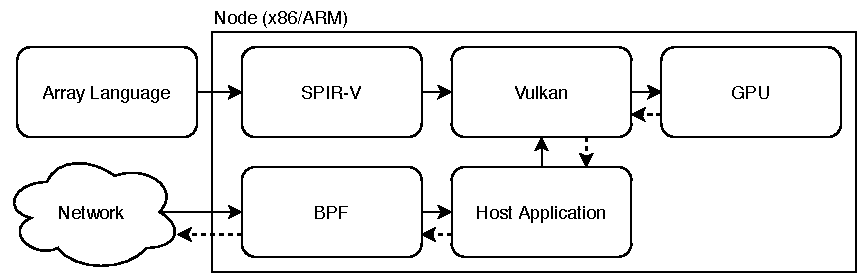
\includegraphics[width=\columnwidth]{system}
  \caption{An envisioned software stack of a GPU node.}
  \label{fig:system}
\end{figure}

Similar to previous \gls{NFV} approaches, such as Netbricks \cite{panda2016netbricks}, in this study, our microservice architecture leverages Rust programming language. Further, also similar to Netbricks, we run the \glspl{NF} unvirtualized. Here, we leverage low-level Vulkan \gls{API} bindings to allow us to refine the GPU computation pipeline to accustom to performance. To elaborate, we declare static resources that exist along the complete lifetime of the program, with other parts, such as program loading, working in a dynamic manner (see: left side of Fig. \ref{fig:vulkan}). Next, to allow GPU NFs to be orchestrated, we integrate our Rust-loader application with Kubernetes Service abstractions (see: Fig. \ref{fig:svc}). In particular, the novelty of our approach here comes from the fact that SPIR-V kernels can be inlined within Kubernetes Service abstraction as string-valued metadata. This is possible because SPIR-V kernels are small in size: our RF prediction algorithm weights in at 2kb without compression. Furthermore, we achieve a non-virtualized and non-container approach while still managing to leverage Kubernetes APIs by defining the GPU nodes inherently as non-schedulable (by not having \gls{CRI} installed, see: Fig. \ref{fig:k8s}) and the Service abstractions as services without selectors. This way, we achieve two things: 1) Kubernetes does not try to schedule any existing worker nodes (for software stack, see: Fig. \ref{fig:system}) to spawn containers for the GPU Services as the Service declarations lack selectors, and 2) the Services are still exposing as a cluster-wide \gls{DNS} entry. This keeps our proposed approach non-invasive to existing Kubernetes installations. Hence, we believe that our proposal to orchestrate GPU NFs this way can be practically viable. The major benefit of integrating with the standard Kubernetes scheduling workflow, orientated around the Service abstraction, is that the GPU Services in our proposed architecture is automatically seen, routed, and exposed within the cluster as any other standard container-based service. This way, we can heavily simplify our loader program: \gls{CNI} handles the networking, CoreDNS the routing, and etcd the kv-storage. For example, for better networking performance, CNI integrations like Cilium can be used to automatically benefit from kernel-passthrough technology \gls{BPF}. Such an approach might be useful when running the GPU NFs on the edge of the network, providing even lower latency to data inference or simply to gain higher packet throughput. The following subsections are meant to further detail and visualize our proposed approach.

\subsubsection{Kubernetes Integration}
\label{ch:k8s}

As mentioned, Kubernetes \cite{burns2016borg} is an orchestrator system for containers, and can be considered as a system which conglomerates multiple physical servers into a single abstracted computing unit. Kubernetes is designed to schedule software packaged into containers, but due to its modular design, it can be retrofitted to also serve other purposes. In this study, we propose a way to retrofit Kubernetes to orchestrate GPU microservices in a cluster, which can also do containers in the traditional way. As such, we consider our approach "non-invasive", as we do not limit the functionality of the standard installation.

\begin{figure}
  \centering
  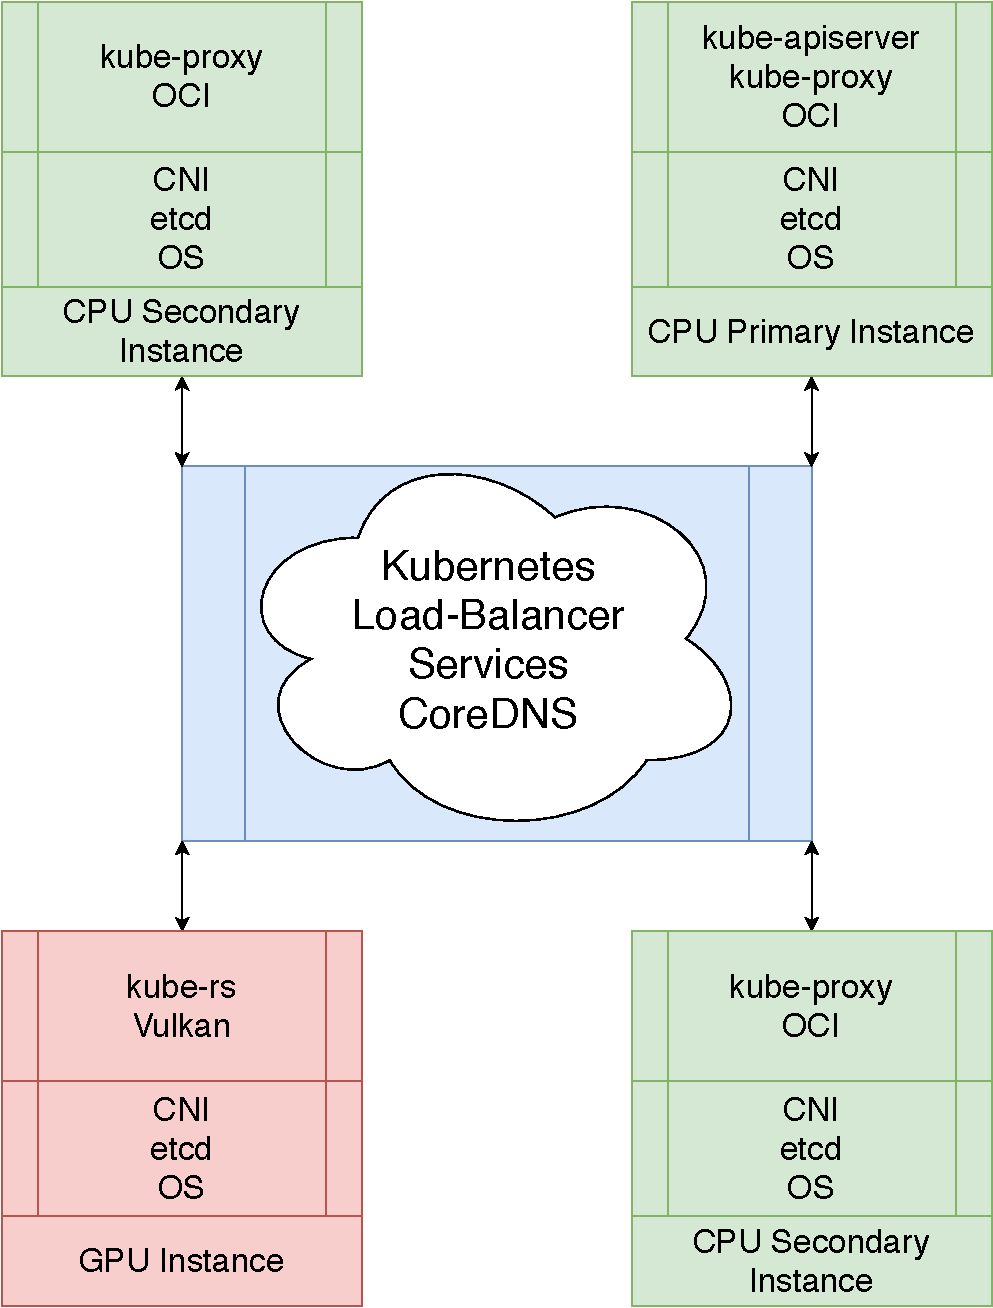
\includegraphics[width=\columnwidth]{k8s2.pdf}
  \caption{Kubernetes integration. Here, four instances form the Kubernetes abstraction. Green instances are container-schedulable, the red one is not.}
  \label{fig:k8s}
\end{figure}

Due to Kubernetes' modular design, the architecture of each installation may vary. In our study, we propose a barebone installation without making too many assumptions about what the underlying modules are. To illustrate our idea, we consider a network topology of a four-node system, in which we have one primary node and three secondaries (pictured in Fig. \ref{fig:k8s}). Here, of the three secondaries, two of them are container hosts, whereas one of them is a GPU host. We propose that the GPU host remains non-schedulable for containers, per arguments regarding NF performance (e.g., see \cite{panda2016netbricks}). On the cluster level, we do not simply cordon the GPU hosts, but instead, never install a \gls{CRI} on the host. This is a possible solution when the Kubernetes cluster installation is done manually (e.g., per instructions of \cite{kelsey}). However, even though the GPU instance is unuseful hence in a sense redundant for the cluster for running containers, it may still be part of the cluster as long as it has the \gls{CNI} installed properly. The CNI is just another module on the Kubernetes stack and can be, e.g., \verb|flannel| or something else. The CNIs then rely on \verb|etcd| which is a distributed kv-storage and one of the most basic requirements for a Kubernetes instance. We insist on the fact that in our proposed architecture, the CNI, CRI and the GPU host operating system may be whatever, as the software stack does not need to be opinionated thanks to the modular interface provided by Kubernetes (to a stark difference, e.g., in Legate \cite{bauer2019legate} where the software stack must be based on proprietary Nvidia stack).

Once these basic services are installed on each node, they should provide a DNS layer for proper addressing withing the cluster. Usually, this is done via CoreDNS as it has a Kubernetes integration, but may also be some other DNS server. Relevant to our proposal, the DNS server is required to correctly route Kubernetes Services, which is the main interface our proposed architecture needs. To quote the Kubernetes documentation, a Service is "an abstraction which defines a logical set of Pods and a policy by which to access them (sometimes this pattern is called a micro-service)". In other words, Service is the Kubernetes-native way of defining a microservice. As such, it is logical for our proposal on the orchestration of GPU NFs as microservices to interface with the Service abstraction.

\begin{figure}
\begin{minipage}[t]{0.45\columnwidth}
\begin{lstlisting}
apiVersion: v1
kind: Service
metadata:
  name: my-service
spec:
  selector:
    app: MyApp
  ports:
    - protocol: TCP
      port: 80
      targetPort: 9376
\end{lstlisting} 
\end{minipage}
\begin{minipage}[t]{0.45\columnwidth}
\begin{lstlisting}
apiVersion: v1
kind: Service
metadata:
  name: my-service
  spirv: AwIjBwAFAQAAAAcAWAAAAAAA...
  binding_count: 7
spec:
  ports:
    - protocol: TCP
      port: 80
      targetPort: 9376
---

apiVersion: v1
kind: Endpoints
metadata:
  name: my-service
subsets:
  - addresses:
      - ip: 192.0.2.42
    ports:
      - port: 9376
\end{lstlisting} 
\end{minipage}
\caption{Kubernetes Service declarations. On the left, one with selectors, which would spawn container image MyApp. On the right, a Service without a selector, which would not spawn any containers. Our proposal uses the right-hand side version to spawn GPU NFs as microservices.}
\label{fig:svc}
\end{figure}

Yet, we do not use the standard declaration of Service, because we do not want to run the GPU NF microservices inside of a container. To elaborate, using containers for GPU applications is tricky and opinionated. For reference, the Kubernetes documentation on using GPUs\footnote{\url{https://kubernetes.io/docs/tasks/manage-gpus/scheduling-gpus/}} lists that to use, e.g., Nvidia GPUs, the cluster has to: 1) have Nvidia drivers pre-installed, 2) have nvidia-docker installed (which only works on Linux), 3) use Docker as the CRI. For AMD, the steps include similar tweaks, including allowing the nodes to run in a privileged mode. In essence, these approaches limit the flexibility of the GPU node installations and require dangerous execution modes for containers, which are usually meant to run in an unprivileged mode. We note that in our proposal, drivers still have to be installed, in addition to Vulkan, but our proposal allows the GPU nodes to remain operating system and CRI agnostic. We achieve this by declaring the Service abstraction without a node selector. To compare these declarations, consider Fig. \ref{fig:svc}. Further, for the Service not to remain orphan, we must declare an Endpoint abstraction manually. This can be done in a single command by separating the configuration declarations with three dashes, as shown in Fig. \ref{fig:svc}.

As can be seen on Fig. \ref{fig:svc}, our proposal for declaring GPU microservices within Kubernetes requires the SPIR-V binary file to be inlined within the metadata description. In our initial proposal, we do not compress the binaries, and the binaries are encoded in base64. Also, the binding count has to be included, which defines how many buffers the SPIR-V kernel includes. The buffers in our initial proposal are always defined as Vulkan Storage Buffers with the Compute type.

After the creation of the Service file, CoreDNS triggers a CNAME entry creation for the Service. We clarify that this is a standard procedure in Kubernetes, which is automatically triggered on Service creation. By default, this would expose an endpoint by name \verb|my-service.default.svc.cluster.local| in each of the cluster's nodes' routing table. In our proposal, what follows is that the Service creation events would be listened by the GPU nodes using a Kubernetes client-wrapper, e.g., \verb|kube-rs|. This means that each GPU node is listening to the primary Kubernetes node to announce changes in the cluster Service entries. One such is found, the GPU nodes would pull the declarations using the HTTP API. This would reveal the SPIR-V binary encoded in base64 and the number of buffer bindings that have to be created for this particular GPU microservice. Finally, if the Endpoints include the node-local IP address, the microservice is provisioned using the Vulkan API. Once the microservice is initialized, the according to port found in the Service declaration is opened on the node. When the port receives packets, the contents are unmarshaled to 1D vector array buffers in Rust and passed to GPU. Once done, the result is written back to the connection which it came from. As such, it is the responsibility of the Kubernetes CNI to route data in and out. Such reliance cuts two ways: on the one hand, our proposal only works with Kubernetes. But on the other hand, we do not make assumptions about what the Kubernetes installation has to be like. As such, it is possible to leverage Kubernetes abstractions on top of the GPU NFs, such as LoadBalancer, to balance the load among many GPU nodes or any other networking constructs. For example, to create a function-chain of NFs, we would encourage the chaining to be declared on Kubernetes-level. This way, the function-chain may mix both GPU NFs and CPU NFs by interfacing via CNAME entries. As such, we consider that our proposal can be used to introduce GPU NFs and other microservices as part of a heterogeneous system consisting of CPU and GPU nodes.

\subsubsection{Vulkan-based Loader Program}
\label{ch:loader}

Our Vulkan-based loader program (see: \ref{fig:vulkan} and high-performance computing and software engineering level contribution on \ref{fig:ov}) uses a Rust-wrapper library called \verb|ash|\footnote{\url{https://github.com/MaikKlein/ash}} to interface with the GPU. In the abstract, \verb|ash| provides conveniences, e.g., wrapping returned structures in vectors, and providing default values for all API call structures. It is also a very low-level in the sense that all operations are "unsafe", which essentially means that the programmer must consult the official Vulkan API documentation to avoid undefined behavior. Coincidentally, this means that the Rust compiler is less useful than usually in respect of memory safety: unsafe calls are meant as code blocks in which the programmer surpasses the type system, and everything in \verb|ash| is unsafe.

In Fig. \ref{fig:vulkan} we demonstrate the program flow of the loader. We start from declaring static variables, i.e., ones which extend to the complete lifetime of the program. Once these are initiated, the shader modules and pipeline layouts of the shaders are retrieved from Kubernetes using a Rust client library to Kubernetes called \verb|kube-rs|\footnote{\url{https://github.com/clux/kube-rs}}. This could be considered as analogous to pulling a container image from a registry to be ready-to-deploy. After this initialization, we open the ports specified by the Kubernetes Services and start waiting for input to the kernels. Once input is received, it goes through a standard Vulkan compute pipeline, which we have detailed step-by-step in the aforementioned figure. In the final step, once the result is copied back to CPU memory, the result is written back to the network socket specified by the Kubernetes Service file. Here on, it is the job of Kubernetes CNI to forward the response to wherever. As such, it could be argued that this way, our approach yields itself well to the working principles of chained NFs, allowing such constructs to be modeled in Kubernetes, possibly spanning multiple Services with GPU NFs and traditional CPU containers complementing each other. Further, we yield to the fact there should exist more performant ways to traverse the Vulkan pipeline -- understanding Vulkan to use it in the most effective way is a subject of many books, thus effectively out-of-scope of what could have been prepared for this study. As such, further pipeline optimizations are left for future studies.

\begin{figure*}
  \centering
  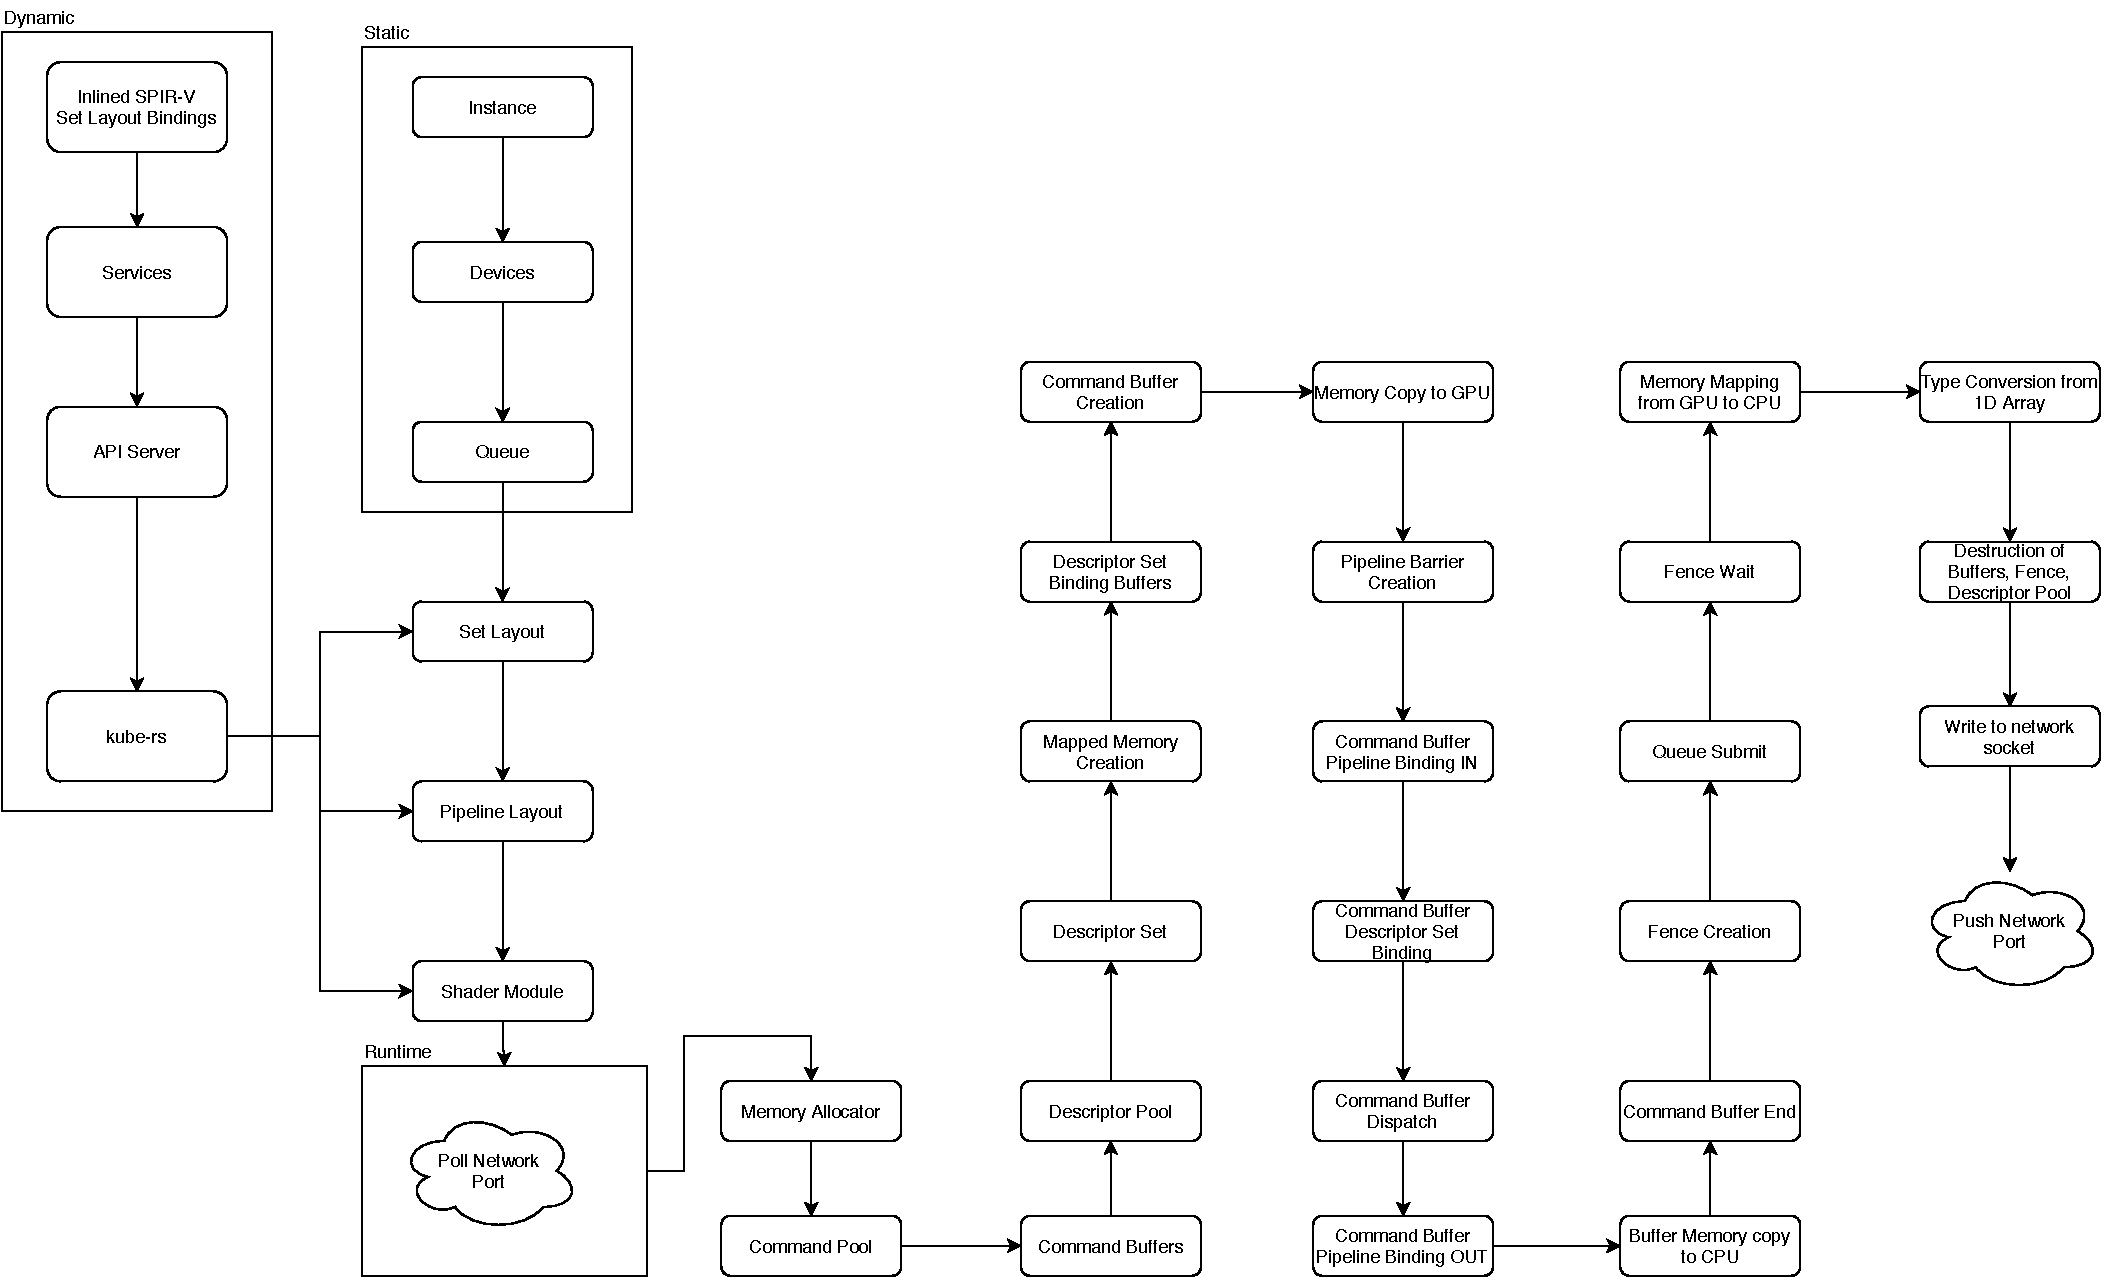
\includegraphics[width=\columnwidth*2]{vulkan3.pdf}
  \caption{Vulkan loader in a nutshell.}
  \label{fig:vulkan}
\end{figure*}

\subsection{Results}
\label{ch:results}

\begin{figure}
  \centering
  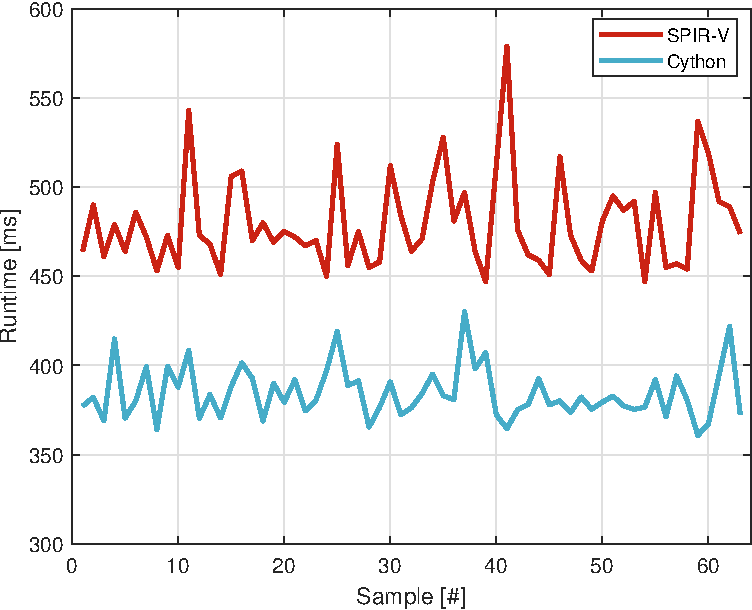
\includegraphics[width=\columnwidth]{bench.pdf}
  \caption{Runtime comparison of random forest model of 150x6000x300 trees between Cython and SPIR-V.}
  \label{fig:bench}
\end{figure}

The benchmarks were run on an Intel i7 processor and Nvidia GTX 2080 GPU. As introduced previously, the application was a \gls{RF} prediction over 150x6000x300 dimensional trees (i.e., quite small). As shown in Fig. \ref{fig:bench}, the Cython code on OpenMP was faster than the GPU code: the average runtime of the Cython code was 380ms (8 cores, 6000 threads) while the SPIR-V took on average 480ms (1024 cores) to execute. Further, the performance variance on the GPU was higher than on the Cython code.

However, even though the GPU code was slower, we estimate that there exists future work in making the GPU approach faster. In specific, due to the time limits of our research, each data buffer is copied separately to the GPU. While the dataset is not big (our dataset weights in at 70MB in total), the memory copies happen sequentially. Yet, it is possible to use Vulkan's fine-grained performance primitives to structure the data in such a way that a single memory copy would suffice. Similarly, garbage collection of the Vulkan resources could be done asynchronously, whereas currently, the operations block each tree iteration. Furthermore, the data structure of the binary decision tree could be reformatted into a path matrix \cite{hsu2016key}. Such a parallel data structure would allow the GPU to use its y-dimension cores when traversing the tree. 

Altogether, we think these results are promising. GPUs are oftentimes thought to only be practical approach after a certain threshold is met, but here we show it can be almost comparable to CPU performance even for small datasets.

\section{Discussion and Future Work}
\label{ch:dicussion}

In our case-study in Section §\ref{ch:contribution} we relied on a hand-coded SPIR-V program. But what about compiling APL straight to SPIR-V and automatically creating the Kubernetes manifest files? According to our research, such is possible but does not come without its challenges. First, the problem considers the well-researched subject of the static compilation of APL. We found that as of recent, the matter has been studied in \cite{slepak2014array} (2014). It seems the work continues with two new pre-prints appearing in 2019 \cite{slepak2019semantics, shivers2019introduction}. In abstract, these papers introduce a new language that leverages dependant types to achieve static rank polymorphism. Meanwhile, in \cite{gibbons2017aplicative} argument is made against inventing a new language. In \cite{gibbons2017aplicative}, the author argues for using Haskell to implement a type checker for static rank polymorphism and provides proof that the issue of type checking APL is possible given the current state of programming language theory and its tools.

Next, we detail why the type checking is important in the context of our goals: one unique challenge GPU environments introduce over the CPU is the non-existence of shared stack memory and inability to allocate memory at runtime. As such, for a generic compiler, the compiler would need to infer the intermediate types after each operation step until program termination. Interestingly, this would also imply that the problem touches on so-called static memory management, which has been an issue in recent programming language research (e.g., \cite{proust2017asap}). To elaborate on the problem, let us suppose the following program:

{\aplfont\begin{verbatim}
⍒ 4 4 ⍴ ?⍳16
\end{verbatim}}

which produces depending on randomness, e.g.,

{\aplfont\begin{verbatim}
3 4 2 1
\end{verbatim}}

I.e., create a random list of 16 integers, reshape them into 4x4 matrix, and for each row of the matrix, sum the values together, and rank then according to the sum value from highest to lowest.

When this program is given to the loader program, the problem is that the buffer dimensions inferred from the initial argument (index of) 16 are not relevant considering the output (of shape 4). This is a problem because the output buffer has to be allocated prior to program execution, meaning that, what would be loaded from the GPU memory would be: 3 4 2 1 0 0 0 0 0 0 0 0 0 0 0 0. This is a false result and would need to be either reshaped on the GPU or the CPU, but regardless of which hardware it is done, the type inference (more precisely in APL terms, the shape inference) has to be known prior to the execution of the kernel (to clear out the unneeded numbers). Yet, the only way to know the final shape of the array is to make a type of inference of the whole program as most APL interpreters are made for CPU hardware they do not concern type inference prior to the runtime as they are able to allocate shared stack memory.

In addition, because of the rho which transforms the list of 16 numbers into a 4x4 matrix, which is then graded down using the indices sort function, we are also introduced to an intermediate problem: the sorting needs to be applied to a shared matrix (as sorting is data-dependant on other threads values), but the matrix has no physical mapping, nor is it the output of the program. To our current knowledge, there are two apparent options to handle this:

\begin{enumerate}

\item Infer the matrix transformation prior to execution and allocate an "intermediate" physical global work buffer Q, which is given as the target memory to the reshape function. This would mean that there are three memory allocations: one for the input (1x16, class CPU-GPU), one for the reshape (4x4, class GPU-only), and one for the output (1x4, class GPU-CPU). Now, the reshape would map the memory into a 4x4 device-class storage buffer, which could then be manipulated using the Y dimension invocation identifier. Hence, this would mean that the Y dimension of the workgroup should always be at least the maximum of any intermediate shapes' Y dimension.

\item Infer the matrix transformation prior to execution, and either allocate or use any "old" memory buffer layouts (memory buffers which do not hold any data-dependency to forthcoming executions) to fit the data into. In this example, the input buffer (1x16, class CPU-GPU) would fit our whole matrix if laid into a one-dimensional format. Also, the input buffer has served its purpose (the program does not need it anymore), so the memory in there would be safe to overwrite. Now, the reshape would map the memory by using a stride identifier of 4. This means, that even though the matrix is handled in a one-dimensional array, the SPIR-V would keep an additional variable in-memory to know that depending on the X dimension invocation identifier, that it is not supposed to use the indices sort beyond the stride. For example, if the invocation ID is 14, this ID could be divided by the stride to infer the "logical" Y dimension of the array. As a benefit, the stride could be coded as a function-local variable within the compilation, hence saving access or allocation in global memory. So, with this approach, it would mean that there are two memory allocations: one for the input (1x16, class CPU-GPU), and one for the output (1x4, class GPU-CPU). The memory usage has decreased, but this method would two-step of one very complicated thing: identify orphan memory + use it such that it can fit the memory (what about if the orphan memory is 3x10? it fits but not exactly, requires more complex stride logic).

\end{enumerate}

Yet, the 2) is logically an improvement over the 1), and 1) would be required at all times: if there simply will not be eligible orphan memory, or it is too small, then memory allocation should be inferred to the principle of 1).

However, this is good to think as it relates closely to the way the information is fed to the GPU: even though it would be possible to define input buffers to already adhere to a matrix or vector dimensions, it might be limiting (and slowing) factor if the original memory layout is probed to be re-used.

A second aspect that would improve from the application of computer science theory is the memory safety of the programs. The more complicated the APL operands become, the more error-prone it is to prove that the algorithms do what they are supposed: GPU programs are parallel constructs, and hence may act nondeterministically. This act is further complicated by the way the memory has to be handled as pointers in the program state -- pointers are generally known to be a very error-prone concept. We stipulate that in the future the APL operands of which the compiler stitches together should either be verified with a model checker to avoid concurrency bugs, or, e.g., use some form of separation logic to make sure that certain parts of the program hold invariants.

As the bottom line, we deem it interesting to next apply proper computer science logic to our contribution: the arguably at-times hacky approach to combine many aspects of system sciences together in this study seems to be ripe to be improved by formalism next. Further, it may well be that due to relation with high-performance computing, the results found in later studies might be practically viable, especially given the fact that should the aforementioned Kubernetes approach be presented as a software plugin rather than mere textual description.

\section{Conclusion}
\label{ch:conclusion}

This study was conducted in the context of NFV, which seeks to replace purpose-built network hardware with commodity hardware such as GPUs. In this study, we used rank polymorphic programming language APL as a parallel modeling language for SPIR-V IR GPU code. In general, we studied how APL could work as a compiled GPU DSL for NFV. Hence, we introduced a way to deploy GPU code written this way to Kubernetes. We also benchmarked an NFV ML application: we timed RF tree prediction of size 150x6000x300 between CPU and GPU. We found that OpenMP powered Cython code on CPU was, on average, 26\% faster than our hand-written Vulkan SPIR-V GPU code. We remark that the benchmark does favor the CPU over GPU due to the small size of the RF tree. We also suggest performance improvements to our GPU implementation. We also discuss challenges and opportunities for extending the APL DSL with type inference. As a conclusion, given the groundwork done in this study, we consider such future work prosperous. In specific, future work would provide novel yet practical features to NFV via ease of programming and verifiable memory consumption policies.

{\renewcommand*{\bibfont}{\small}\printbibliography}

\newpage

\appendix
\section{Full APL code}

\begin{figure}
  \centering
  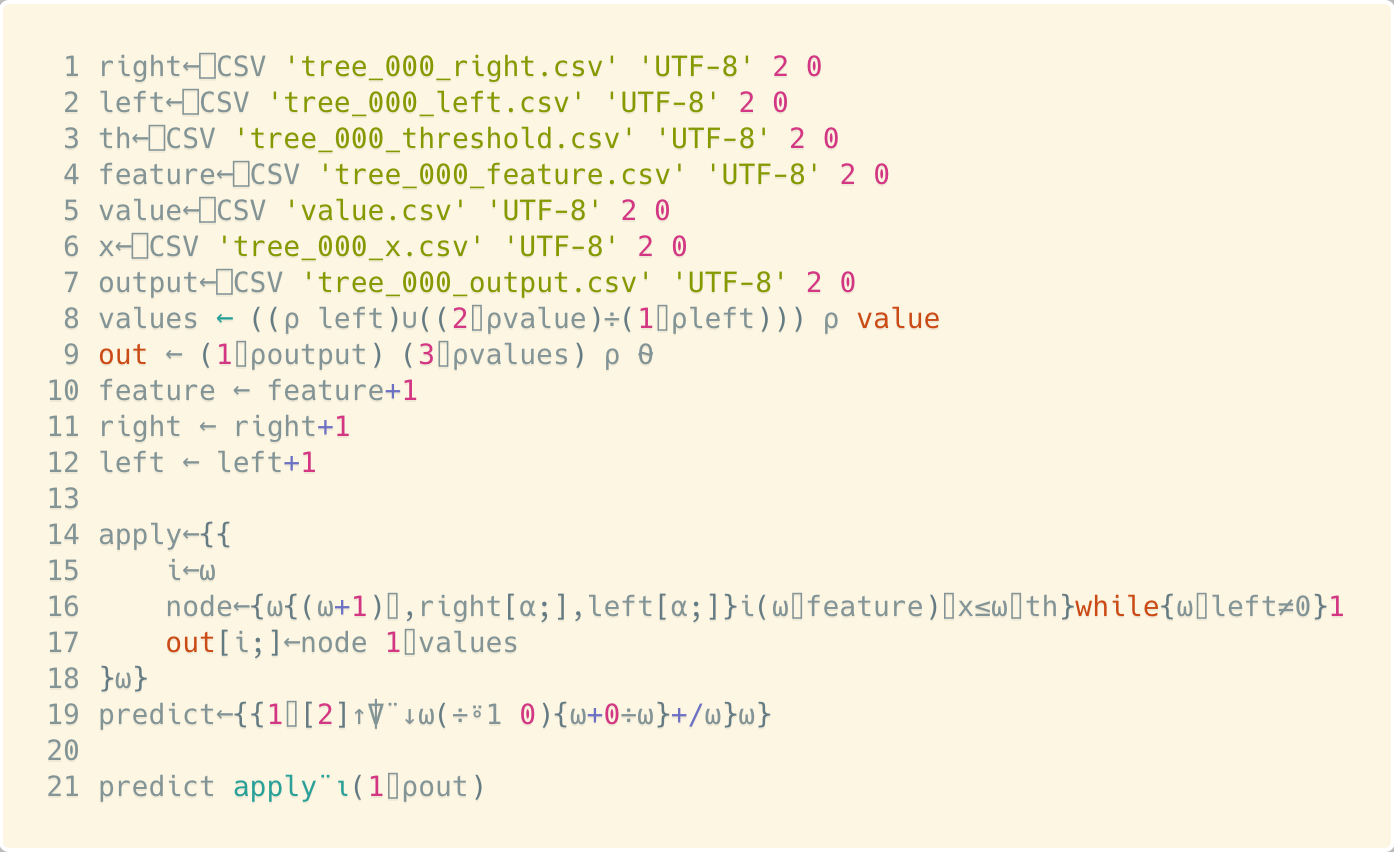
\includegraphics[width=\columnwidth]{aplsrc.png}
  \caption{APL refactor of the Python source code.}
  \label{fig:aplsrc}
\end{figure}

Due to the font-problems of LaTeX, we present the multiline source-code of APL as Fig. \ref{fig:aplsrc} instead of textual representation.

\section{SPIR-V SSA code}
\begin{lstlisting}
; SPIR-V
; Version: 1.5
; Generator: Khronos SPIR-V Tools Assembler; 0
; Bound: 85
; Schema: 0
               OpCapability Shader
               OpCapability VariablePointers
               OpCapability VulkanMemoryModel
               OpMemoryModel Logical Vulkan
               OpEntryPoint GLCompute %1 "main" %gl_GlobalInvocationID %3 %4 %5 %6 %7 %8 %9
               OpExecutionMode %1 LocalSize 1024 1 1
               OpDecorate %gl_GlobalInvocationID BuiltIn GlobalInvocationId
               OpDecorate %_arr__arr_float_uint_198_uint_5788 ArrayStride 792
               OpMemberDecorate %_struct_11 0 Offset 0
               OpDecorate %_struct_11 Block
               OpDecorate %3 DescriptorSet 0
               OpDecorate %3 Binding 0
               OpDecorate %3 Aliased
               OpDecorate %_arr_float_uint_3285 ArrayStride 4
               OpMemberDecorate %_struct_13 0 Offset 0
               OpDecorate %_struct_13 Block
               OpDecorate %4 DescriptorSet 0
               OpDecorate %4 Binding 1
               OpDecorate %5 DescriptorSet 0
               OpDecorate %5 Binding 2
               OpDecorate %6 DescriptorSet 0
               OpDecorate %6 Binding 3
               OpDecorate %7 DescriptorSet 0
               OpDecorate %7 Binding 4
               OpDecorate %_arr_float_uint_198 ArrayStride 4
               OpDecorate %_arr__arr_float_uint_198_uint_3285 ArrayStride 792
               OpMemberDecorate %_struct_16 0 Offset 0
               OpDecorate %_struct_16 Block
               OpDecorate %8 DescriptorSet 0
               OpDecorate %8 Binding 5
               OpDecorate %_arr_float_uint_300 ArrayStride 4
               OpDecorate %_arr__arr_float_uint_300_uint_5788 ArrayStride 1200
               OpMemberDecorate %_struct_19 0 Offset 0
               OpDecorate %_struct_19 Block
               OpDecorate %9 DescriptorSet 0
               OpDecorate %9 Binding 6
       %uint = OpTypeInt 32 0
        %int = OpTypeInt 32 1
       %void = OpTypeVoid
         %23 = OpTypeFunction %void
       %bool = OpTypeBool
      %float = OpTypeFloat 32
   %uint_300 = OpConstant %uint 300
  %uint_5788 = OpConstant %uint 5788
  %uint_3285 = OpConstant %uint 3285
   %uint_198 = OpConstant %uint 198
     %v3uint = OpTypeVector %uint 3
%_ptr_Input_v3uint = OpTypePointer Input %v3uint
%gl_GlobalInvocationID = OpVariable %_ptr_Input_v3uint Input
%_ptr_Input_uint = OpTypePointer Input %uint
%_arr_float_uint_3285 = OpTypeArray %float %uint_3285
 %_struct_13 = OpTypeStruct %_arr_float_uint_3285
%_ptr_StorageBuffer__struct_13 = OpTypePointer StorageBuffer %_struct_13
          %4 = OpVariable %_ptr_StorageBuffer__struct_13 StorageBuffer
          %5 = OpVariable %_ptr_StorageBuffer__struct_13 StorageBuffer
          %6 = OpVariable %_ptr_StorageBuffer__struct_13 StorageBuffer
          %7 = OpVariable %_ptr_StorageBuffer__struct_13 StorageBuffer
%_arr_float_uint_198 = OpTypeArray %float %uint_198
%_arr__arr_float_uint_198_uint_3285 = OpTypeArray %_arr_float_uint_198 %uint_3285
 %_struct_16 = OpTypeStruct %_arr__arr_float_uint_198_uint_3285
%_ptr_StorageBuffer__struct_16 = OpTypePointer StorageBuffer %_struct_16
          %8 = OpVariable %_ptr_StorageBuffer__struct_16 StorageBuffer
%_arr_float_uint_300 = OpTypeArray %float %uint_300
%_arr__arr_float_uint_300_uint_5788 = OpTypeArray %_arr_float_uint_300 %uint_5788
 %_struct_19 = OpTypeStruct %_arr__arr_float_uint_300_uint_5788
%_ptr_StorageBuffer__struct_19 = OpTypePointer StorageBuffer %_struct_19
          %9 = OpVariable %_ptr_StorageBuffer__struct_19 StorageBuffer
%_arr__arr_float_uint_198_uint_5788 = OpTypeArray %_arr_float_uint_198 %uint_5788
 %_struct_11 = OpTypeStruct %_arr__arr_float_uint_198_uint_5788
%_ptr_StorageBuffer__struct_11 = OpTypePointer StorageBuffer %_struct_11
          %3 = OpVariable %_ptr_StorageBuffer__struct_11 StorageBuffer
%_ptr_Function_uint = OpTypePointer Function %uint
%_ptr_StorageBuffer__arr_float_uint_198 = OpTypePointer StorageBuffer %_arr_float_uint_198
%_ptr_StorageBuffer_float = OpTypePointer StorageBuffer %float
%_ptr_Function_float = OpTypePointer Function %float
     %uint_0 = OpConstant %uint 0
     %uint_1 = OpConstant %uint 1
     %int_n1 = OpConstant %int -1
    %float_0 = OpConstant %float 0
   %float_n1 = OpConstant %float -1
         %46 = OpTypeFunction %uint %uint
          %1 = OpFunction %void None %23
         %47 = OpLabel
         %48 = OpAccessChain %_ptr_Input_uint %gl_GlobalInvocationID %uint_0
         %49 = OpLoad %uint %48
         %50 = OpULessThan %bool %49 %uint_5788
               OpSelectionMerge %51 None
               OpBranchConditional %50 %52 %53
         %52 = OpLabel
         %54 = OpFunctionCall %uint %55 %49
         %56 = OpAccessChain %_ptr_StorageBuffer__arr_float_uint_198 %3 %uint_0 %49
         %57 = OpAccessChain %_ptr_StorageBuffer__arr_float_uint_198 %8 %uint_0 %54
         %58 = OpLoad %_arr_float_uint_198 %57
               OpStore %56 %58
               OpBranch %51
         %53 = OpLabel
               OpBranch %51
         %51 = OpLabel
               OpReturn
               OpFunctionEnd
         %55 = OpFunction %uint None %46
         %59 = OpFunctionParameter %uint
         %60 = OpLabel
         %61 = OpVariable %_ptr_Function_uint Function %uint_0
               OpBranch %62
         %62 = OpLabel
               OpLoopMerge %63 %64 None
               OpBranch %65
         %65 = OpLabel
         %66 = OpLoad %uint %61
         %67 = OpAccessChain %_ptr_StorageBuffer_float %4 %uint_0 %66
         %68 = OpLoad %float %67
         %69 = OpConvertFToS %int %68
         %70 = OpINotEqual %bool %69 %int_n1
               OpBranchConditional %70 %71 %63
         %71 = OpLabel
         %72 = OpAccessChain %_ptr_StorageBuffer_float %7 %uint_0 %66
         %73 = OpLoad %float %72
         %74 = OpConvertFToU %uint %73
         %75 = OpAccessChain %_ptr_StorageBuffer_float %9 %uint_0 %59 %74
         %76 = OpLoad %float %75
         %77 = OpAccessChain %_ptr_StorageBuffer_float %6 %uint_0 %66
         %78 = OpLoad %float %77
         %79 = OpFOrdLessThanEqual %bool %76 %78
         %80 = OpSelect %_ptr_StorageBuffer__struct_13 %79 %4 %5
         %81 = OpAccessChain %_ptr_StorageBuffer_float %80 %uint_0 %66
         %82 = OpLoad %float %81
         %83 = OpConvertFToU %uint %82
               OpStore %61 %83
               OpBranch %64
         %64 = OpLabel
               OpBranch %62
         %63 = OpLabel
         %84 = OpLoad %uint %61
               OpReturnValue %84
               OpFunctionEnd
\end{lstlisting}

\end{document}
